\documentclass[a4paper,12pt]{article}
  %\documentclass[a4paper,10pt]{scrartcl}

\usepackage[utf8]{inputenc}
\usepackage{amsmath}
\usepackage{graphicx}
\usepackage{color}
\usepackage{hhline}
\usepackage{array}
\usepackage{subfigure}
\usepackage[titletoc,title]{appendix}
\usepackage[pdfborder={0 0 0}]{hyperref}
\usepackage{float} 
\usepackage{tabularx}

\newcommand{\HRule}{\rule{\linewidth}{0.5mm}}
\newcolumntype{G}{!{\vrule width 2pt}}
\newlength\savewidth
 \newcommand\Ghline{%
	\noalign{\global\savewidth\arrayrulewidth\global\arrayrulewidth2pt}%
	\hline
	\noalign{\global\arrayrulewidth\savewidth}}



\pdfinfo{%
  /Title    (Automatic biorhythms description from actigraphy data)
  /Author   (Miguel Gonzalez)
  /Creator  (Miguel Gonzalez)
  /Producer (Miguel Gonzalez)
  /Subject  (TFE)
  /Keywords ()
}



\begin{document}
 \begin{titlepage}
\begin{center}


\begin{minipage}[ht]{0.4\textwidth}
\begin{flushleft} \large
\textsc{Miguel GONZALEZ Y VIAGAS}
\end{flushleft}
\end{minipage}
\begin{minipage}[ht]{0.4\textwidth}
\begin{flushright} \large
\textsc{Année académique 2013-2014}
\end{flushright}
\end{minipage}\\[2cm]



\textsc{\LARGE Université de Liège} \\[1cm]
\textsc{\Large Faculté des sciences appliquées} \\[1cm]
\textsc{\large Mémoire de fin d'études réalisé en vue de l'obtention du grade de Master ingénieur civil biomédical} \\[1cm]


\HRule \\[4mm]
\textsc{\Large Description des biorythmes d’une population normale jeune à partir de données actimétriques} \\[1mm]
\HRule \\[3cm]

   \begin{minipage}[c]{.46\linewidth}

\includegraphics[scale=0.2]{Images/logoULg.png}
   \end{minipage} \hfill
   \begin{minipage}[c]{.46\linewidth}

\includegraphics[scale=0.4]{Images/fsa.jpg}
   \end{minipage}


\end{center}
\end{titlepage}

 
 \section*{Acknoledgements}
 
 \paragraph{}
 First, I'd like to thank my promoter, Christophe Phillips. Not only for introducing me to this attractive master's thesis subject but particularly for his constant disponibility and lucid advice during the whole process of my thesis. In the same vein, I thank Sarah Chellappa for help to let me better understand the theoretical part of my subject and for her advices.
 
 \paragraph{}
 Of course, I also want to thank all the teachers that I have crossed during my schooling thanks to whom I've learnt a lot.
 
 \paragraph{}
 I also would like to thank my family as well as my friends for their support during all these years and the relaxing time they offered me during these laborious school years.
 
 \paragraph{}
 Finally, I want to wish a good future to my classmates for professional as well as personnal matters.

\newpage

\section*{}

\begin{center}

\textsc{\Large Automatic biorhythms description from actigraphy data} \\[3mm]

\textsc{\large GONZÀLEZ Y VIAGAS} \large Miguel \\[3mm]

2e année du grade de master en ingénieur civil biomédical \\[5mm]

Année 2013-2014

\end{center}


\paragraph{}
\textbf{Objective:} Manual scoring of regular and successive sleep-wake periods derived from actigraphy is laborious, time-consuming and prone to inter-individual differences across raters. To counteract these current limitations, we developed an automatic algorithm to standardize and fasten this procedure.

\paragraph{}
\textbf{Method:} We used two steps. First, we estimated regular sleep/wake periods (over at least 7 successive days) with classic signal processing. This approach comprised removal of incorrectly timed data and a median filtering with subject-specific thresholding, followed by morphological opening/closing. This leads to rough estimation of final output. In the second step, data and estimations were divided into 5-min windows, labelled as either ‘sleep’ or ‘wake’. Subsequently, a machine learning approach was applied onto these segments, and the trained machine was used to improve scoring. Finally, we compared these results with manual scoring considering 4 major criterions: agreement rate, sensitivity (periods correctly scored as wake over all periods scored as wake), specificity (periods correctly scored as sleep over all periods scored as sleep), and Cohen's kappa.

\paragraph{}
\textbf{Result:} Successive and regular 7-day actigraphy recordings from 25 young healthy participants were scored by an expert and the automatic algorithm. Overall, we obtained an agreement rate of 96.7\%, sensitivity of 96.7\%, specificity of 97.0\% and Cohen's kappa of 92.6\%.

\paragraph{}
\textbf{Conclusion:} Our automatic actigraphy scoring was as good as the manual scoring, as indexed by the high agreement rate and sensitivity/specificity ratios. Importantly, the automatic scoring worked much faster, and is robust and reproducible. Matlab code for these analyses will be freely distributed.
\newpage

 \newpage
 
 \tableofcontents
 \newpage


\section*{Introduction}

\paragraph{}
Over the last few decades, actigraphy has been more and more used in sleep studies. Its low cost combined with its portability and its ease of use have have turned it into a convincing rival to polysomnography, the gold standard in sleep studies. This is supported by the fact that studies have showned that actigraphy is almost as accurate as polysomnography when rating the sleep/wake cycles of individuals.

\paragraph{}
Actigraph units output an activity value for every epoch recorded. The sleep/wake scoring must then be computed from these values. Originally, this scoring was done by hand. A scientist had to look at the data and make an estimation of the scoring. This way of doing has quite a few drawbacks. From the scientist point of view, it is a tedious task: it may take some time and it it not very intellectually demanding. From the precision point of view, it may lead to inaccuracies: the scoring is subjective and it is unlikely that two scientists give the same scoring when analyzing the same actigraphic data.

\paragraph{}
This has lead scientists to look for automatic ways of scoring. Indeed automatic methods would overcome the manual scoring's drawbacks. The aim of these studies is of course to find automatic methods which don't lead to a significant loss in accuracy when compared to manual scoring methods. Automatic methods firstly used ''basic'' signal processing techniques but they have become more and more complex and precise over the years. Some of these automatic algorithms are presented below.

\paragraph{}
Based on these past studies, we developed a new method to score automatically sleep/wake cycles from actigraphic data. First, a preprocessing is applied on the data for them to take the correct format and be usable by the algorithm. Then, the algorithm is applied in two steps. The first step consists of classic signal processing (median filtering, rank-order filtering, ...) and outputs an estimated of the final scoring. The second step consists of a machine learning made on this estimate. The trained machine is then used to perfect the transition times (wake to sleep and sleep to wake). \\
At the end of the paper, the results of our algorithm are presented to ascertain its precision and its usability for future actigraphy studies.

\newpage

\section{Actigraphy}

\paragraph{}
Actigraphy is a method used to monitor the sleep-wake cycles of individuals over one or more successive days. It uses an actigraph unit that consists of a wristwatch-shaped device, which can be worn around the wrist or the ankle. This device contains at least an internal clock, a memory and a piezoelectric movement sensor which can detect movements in up to three dimensions. At regular intervals (defined by the sampling frequency of the device), the electric signal due to the movement is translated to an analogic signal and is stored in the memory. Once enough data has been collected for the study, the actigraph unit is removed from the subject and one can access the activity data by retrieving the data stored in the device's memory. These data are then analyzed manually (by a human scorer) or automatically to retrieve useful data about the circadian cycles of the subject and the quality of his sleep.

\begin{figure}[H]
\centering
\subfigure[Raw activity]{
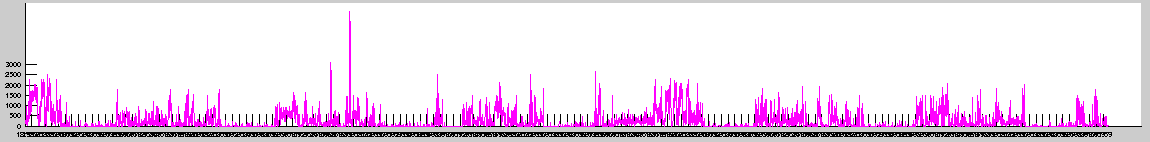
\includegraphics[scale=0.25]{Images/rawActivity.png}}
\subfigure[Sleep-wake scoring performed by a human scorer (blue = wake, white = sleep)]{
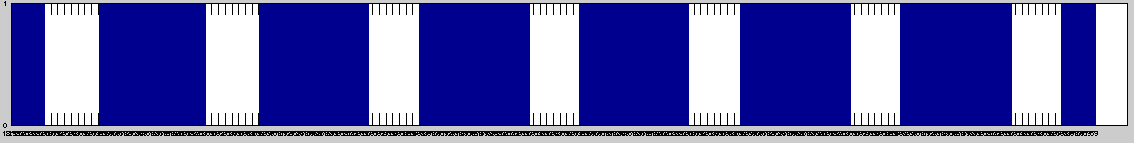
\includegraphics[scale=0.25]{Images/scoring.png}}
\caption{Actigraphic activity of an healthy subject and the corresponding scoring}
\end{figure}

\subsection{The actigraph Unit}

\begin{figure}[H]
\centering
\subfigure[Actigraph wrist watch sensor (from Srinivasan et al. \cite{Srinivasan2010})]{
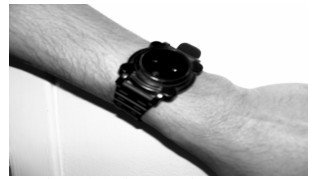
\includegraphics[scale=0.45]{Images/actigraph2.jpg}}
\subfigure[A child sleeping with an actigraph unit attached to her left wrist. (from Sadeh \cite{Sadeh2005})]{
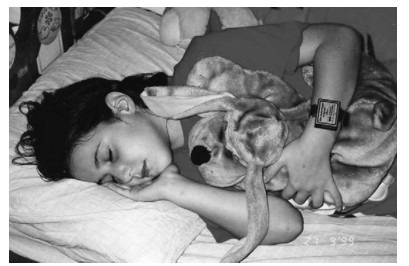
\includegraphics[scale=0.35]{Images/actigraph.jpg}}
\caption{Actigraphy units}
\end{figure}

\paragraph{}
The actigraph unit is a watch-like device which is worn by the subject and will collect the activity data during a certain period of time. Depending on the model, it may be worn around the wrist or around the ankle.

\paragraph{}
Usually, an actigraphy unit is composed of:

\begin{itemize}
\item An accelerometer to detect the activity of the wrist. Some accelerometers~\cite{Pires2009} may detect movements in 3 dimensions while others are only able to detect them in 1 dimension (orthogonal to the device). The accelerometer is bound to an A/D converter to supply a digital output
\item A memory to store the activity data from the accelerometer while it is being used
\item An interface (USB, serial, ...) to download to data from the memory
\item A (rechargeable) battery to power the electrical components in the unit~\cite{LisaJ.MeltzerHawleyE.Montgomery-DownsSalvatoreP.Insana2012} 
\end{itemize}

\paragraph{}
Modern actigraph devices may also contain more features, such as light sensors, off-wrist detectors, etc.~\cite{LisaJ.MeltzerHawleyE.Montgomery-DownsSalvatoreP.Insana2012}

\paragraph{}
For every epoch (i.e. for every minute), a quantification of the subject's activity is stored in the memory. The quantification of this activity is done by using one of these three modes~\cite{Blackwell2008}\cite{Jean-Louis2001} :

\begin{itemize}
\item Zero Crossing (ZC) mode
\item Time Above Threshold (TAT)
\item Proportional Integration (PI)
\end{itemize}

\paragraph{ZC Mode}
In ZC mode, the output value is the sum of the number of times the signal voltage crosses a pre-set zero threshold during the epoch. This zero threshold represents the inactivity state.

\paragraph{TAT Mode}
In TAT mode, the output value is the amount of time (usually in tenths of a second~\cite{Blackwell2008}) spent above a set threshold.

\paragraph{PI Mode}
In PI mode, the output value is the area under the signal (AUC, Area Under the Curve).

\paragraph{}
Fig.~\ref{actiModes2} displays an illustration of the use of the three modes. Fig.~\ref{actiModes1} shows the output when using each of these modes.

\begin{figure}[H]
\centering
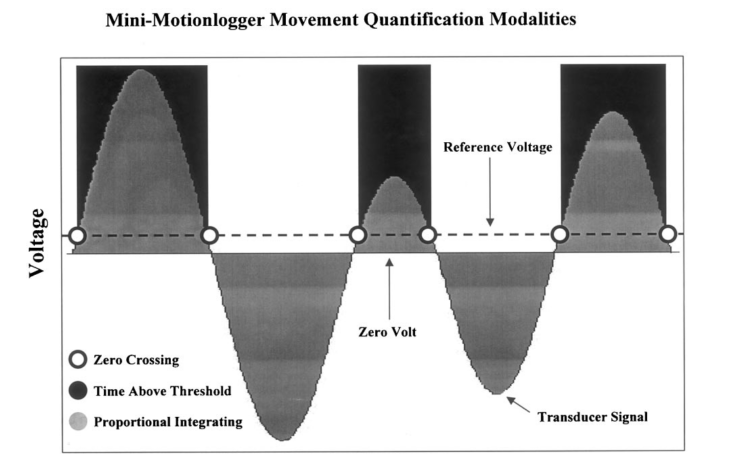
\includegraphics[scale=0.5]{Images/actiModes2.png}
\caption{Diagrammatic illustration of the motion-quantifying modalities of the BASIC Mini-Motionlogger actigraph depicting one epoch of activity emanated from the same transducer signal (from \cite{Jean-Louis2001})}
\label{actiModes2}
\end{figure}

\begin{figure}[H]
\centering
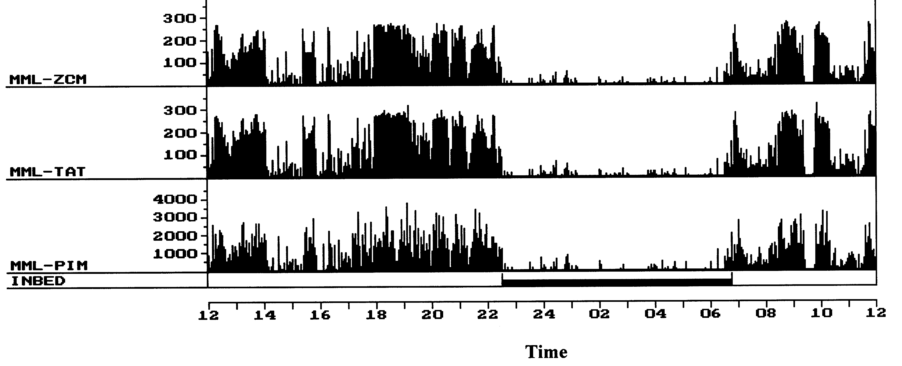
\includegraphics[scale=0.4]{Images/actiModes1.png}
\caption{Plot of activity-rest showing data gathered from two actigraphs worn concomitantly on the same wrist (from \cite{Jean-Louis2001})}
\label{actiModes1}
\end{figure}

\paragraph{}
Although all these three modes provide useful results, Jean-Louis et al.~\cite{Jean-Louis2001}, when studying the different modes of the Mini Motionlogger, found that PI mode was the mode to be ''\textit{favored for determination of sleep-wake states of individuals in the age group studied [mean age=25, SD=6], since accuracy and correlations of PIM estimates were superior to those of the other four quantification modalities}''\cite{Jean-Louis2001}

\paragraph{}
Other modes exist but are less frequent in the litterature, such as SUMACT or MAXACT~\cite{Jean-Louis2001}.

\subsection{Polysomnygraphy}

\paragraph{}
The main other method used in sleep studies is polysomnography (PSG), which is considered as the \textit{gold standard} in sleep studies. PSG is a method that records many body parameters such as Electroencephalography (EEG), Electromyography (EMG), Electrocardiography (ECG) and Electrooculography (EOG). The parameters that are recorded may vary from a study to another.

\paragraph{}
During a study, several electrodes and wires are attached to the subject in order to retrieve all the parameters of interest while the subject is sleeping as depicted on the picture below (Fig.~\ref{PSG}).

\begin{figure}[H]
\centering
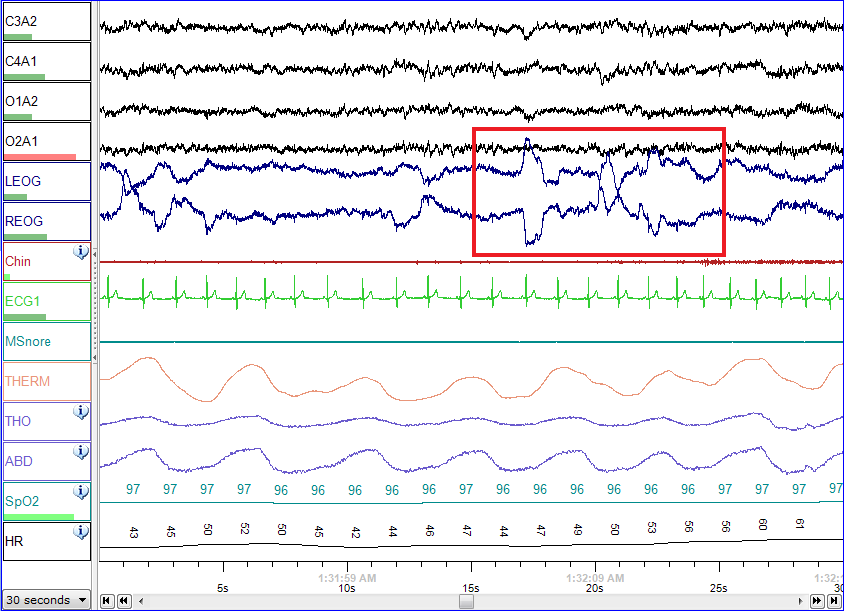
\includegraphics[scale=0.4]{Images/PSG.png}
\caption{PSG record of REM sleep (from wikipedia)}
\end{figure}

\paragraph{}
Even though PSG is the best tool to obtain accurate information about the sleep of the participants, it has some substantial drawbacks :

\begin{figure}[H]
\centering
\begin{tabularx}{\textwidth}{|X|X|X|}
\hline
& PSG & Actigraphy \\
\Ghline
Cost & 5 to 10 times more expensive than actigraphy for the EEG recording system alone~\cite{Mullaney1980} & The only cost is the purchase of the actigraph unit \\
& & \\
Portability & PSG studies must take place in a laboratory which means that the subject is not in his usual environment & Actigraphic studies allow their patients to go back to their home and live a normal life, the only restriction being that the actigraph must be removed while the patient exercise or when he takes a shower. This lets scientists obtain ''real life'' data \\
& & \\
Comfort & As it can be seen on the figure~\ref{PSG}, PSG requires a lot of wire attachments which can be quite uncomfortable for the subject and may alter his sleep & The actigraph unit is more comfortable as it is a simple watch-like device that is worn around the wrist. \\
\hline
\end{tabularx}
\end{figure}

\paragraph{}
Due to these drawbacks, actigraphy will often be prefered over PSG when the sleep-wake schedules needs to be assessed over long periods.

\begin{figure}[H]
\centering
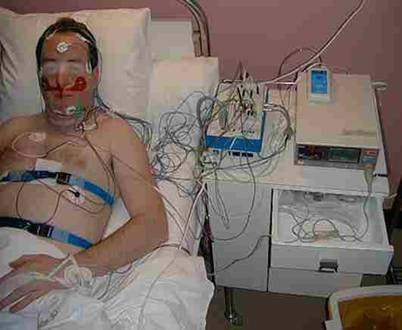
\includegraphics[scale=1]{Images/PSG.jpg}
\caption{Polysomnography (from http://www.labrha.com/fibromyalgie-sommeil-polysomnographie.aspx)}
\label{PSG}
\end{figure}

\subsection{Actigraphy Scoring}

\paragraph{}
Nevertheless, the compensation for the advantages of actigraphy over polysomnography is a loss in the accuracy of the sleep/wake scoring. Mullaney et al.~\cite{Mullaney1980} ran a study to know how less accurate actigraphy was compared to PSG.

\paragraph{}
They worked with 102 recordings including 39 from hospitalized patients which suffered disturbered sleep. During one night, the participants wore an actigraph unit (on the dominant wrist) as well as electrodes used to record EMG, EEG and EOG signals. They were also asked to press a signal marker when going to bed as well as filling a sleep log on the next day about their estimated sleep time and sleep quality.

\paragraph{}
With these data, two scorings were performed: one using the PSG data combined with the sleep logs and the other one using the actigraphy data alone. The two scorings were then compared minute by minute to find the agreement rate. For the 102 recordings, they obtained an agreement rate of $94.5\%$ of all minutes: $96.3\%$ for the healthy controls and $91.6\%$ for the patients.

\paragraph{}
A more interesting measure was also computed: ''the extent to which the wrist actigraphic scoring reflects inter-subject and inter-night variability in Sleep Time''\cite{Mullaney1980}. The correlation coefficient between the two scorings for Total Sleep Time was then computed. They obtained an $r = 0.90 (p < 0.0001)$ which shows that actigraphy reflects most of the variance in PSG Sleep Time.

\paragraph{}
Although these correlations showed that actigraphy was an accurate tool to replace PSG, they found that ''\textit{actigraphic scorer's estimate of TST was, on the average, 15.33 min greater per night than the EEG estimate, and this difference was highly significant ($t = 3.82$, $p < 0.0001$)}''. This comes from the fact that there are occasions when the subject doesn't move his wrist even when he is awake. This was especially noticeable for the patients group of the study.

\paragraph{}
Even though actigraphy scoring is faster and easier than PSG scoring while remaining accurate enough, it still has some important drawbacks:

\begin{figure}[H]
\centering
\begin{tabularx}{\textwidth}{|X|X|}
\hline
& \\
Human ressources & It requires the work of a scientist to manually score the data which could be doing something else \\
& \\
Formation & It requires for this scientist to have a formation on how to score the data properly \\
& \\
Boredom & It is a boring, tedious task that is not really intellectually demanding \\
& \\
Subjectivitiy & It is subjective, therefore scorer-dependent: two different scorers will roughly obtain the same results but they will never be exactly the same \\
& \\
\hline
\end{tabularx}
\end{figure}

\paragraph{}
These are some of the reasons why an automatic way of scoring has been developped. One of the first algorithm was developped by Webster et al.~\cite{Webster1982}. It was a simple technique that used elementary signal processing techniques. Thereof, several new techniques have arisen that use more and more complex processing tools. The aim of all these new techniques is always the same: keeping all the benefits that come with the use of actigraphy while minimizing the loss of accuracy.

\paragraph{}
As actigraphy is more and more frequently used in sleep studies (see Fig.~\ref{actiStudies}), it is an essential task to find automatic scoring methods that are as accurate as possible. Typically, modern studies achieve an agreement rate between they scoring and the gold standard (PSG or human scoring) of $>90\%$\cite{Pires2009}\cite{Crespo2012}.

\paragraph{}
A more detailled presentation of these automatic scoring techniques is illustrated in section ~\ref{sec:stateOfTheArt}.

\begin{figure}[H]
\centering
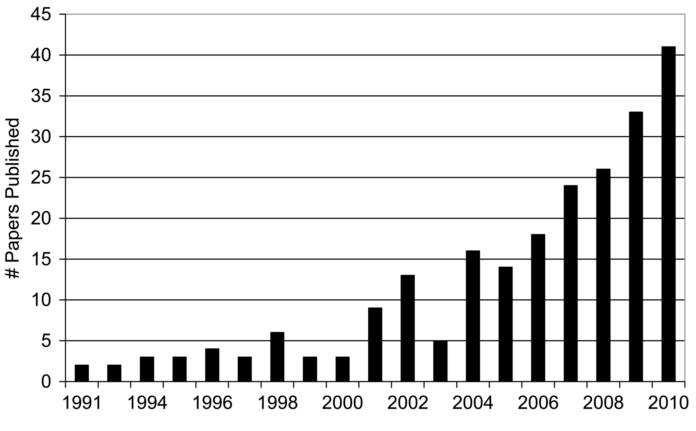
\includegraphics[scale=0.5]{Images/actiStudies.png}
\caption{The number of published research papers that included actigraphy in pediatric populations}
\label{actiStudies}
\end{figure}


%\paragraph{}
%Chae et al.\cite{Chae2009} worked with an Actiwatch-%L\footnote{http://www.jdinstruments.com/actiwatchl.html}. %The software in this device estimated that the subject was asleep %when it encoutered a 10-min window of immobility (at most one %epoch showing some activity). As no explanation were to be found %about the choice of the 10-min window, Chae et al. tried the same %algorithm with other length of windows and found that the window %length that minimized that bias and maximized the correlation %between the actigraphic scoring and the PSG scoring.

\paragraph{}
Finally, in addition to the sleep-wake scoring, the automatic actigraphy scoring methods should be able to provide some parameters of interest in sleep studies. These parameters are frequently met in sleep studies as they are relevant in the determination of the sleep quality of an individual.

\begin{figure}[H]
\centering
\begin{tabularx}{\textwidth}{|X|X|}
\hline
& \\
Sleep Onset & Transition from wakefulness to sleep \\
& \\
Sleep Onset Latency & ''\textit{The interval in minutes from lights-out to the first epoch of any sleep stage without regard to the timing of immobility}''\cite{Chae2009} \\
& \\
Sleep Offset & Transition from sleep to wakefulness \\
& \\
Actual sleep time & Sleep offset - sleep onset \\
& \\
Bed time & Time when the subject goes to bed \\
& \\
Get up time & Time when the subject leaves his bed \\
& \\
Assumed sleep time & Bed time - get up time \\
& \\
Wake After Sleep Onset & The amount of time spent awake between sleep onset and sleep offset \\
& \\
Total Sleep Time & Actual sleep time - WASO \\
& \\
Sleep efficiency & ''\textit{Ratio of TST to total time in bed * 100}''\cite{Paquet2007} \\
& \\
Sensitivity & ''\textit{The proportion of epochs scored as sleep using polysomnography that are accurately identified as sleep by actigraphy.}''\cite{LisaJ.MeltzerHawleyE.Montgomery-DownsSalvatoreP.Insana2012} \\
& \\
Specificity & ''\textit{the proportion of polysomnography-scored wake epochs accurately identified as wake by actigraphy}''\cite{LisaJ.MeltzerHawleyE.Montgomery-DownsSalvatoreP.Insana2012} \\
& \\
\hline

\end{tabularx}


\end{figure}


\subsection{Usage}

\paragraph{}
Jean-Louis et al.~\cite{Jean-Louis1997a} made a study about several issues that may occur when using actigraph units: the ''first-night effect'', the placement of the unit, the sensitivity after extensive use, etc.

\subsubsection{Placement}

\paragraph{}
An important element that must be taken into account is the choice of where to place the actigraph unit on the subject. Firstly, whether it will be worn on the wrist or on the ankle and secondly, whether it will be worn on the dominant wrist/ankle or on the non-dominant one. Intuitively, the dominant wrist seems the most pertinent as it is expected to produce more activity than the non-dominant wrist. This is the reason why the dominant wrist was often chosen in early studies made on actigraphy~\cite{Mullaney1980}. In more modern studies, the non-dominant wrist is usually preferred.~\cite{Crespo2012}\cite{Pires2009}

\paragraph{}
The actigraph units were known~\cite{Sadeh1994} to give different activity outputs according to where they were worn on but Jean-Louis et al.~\cite{Jean-Louis1997a} tried to determine whether the sleep-wake algorithms were robust to these differences or not.

\begin{figure}[H]
\centering
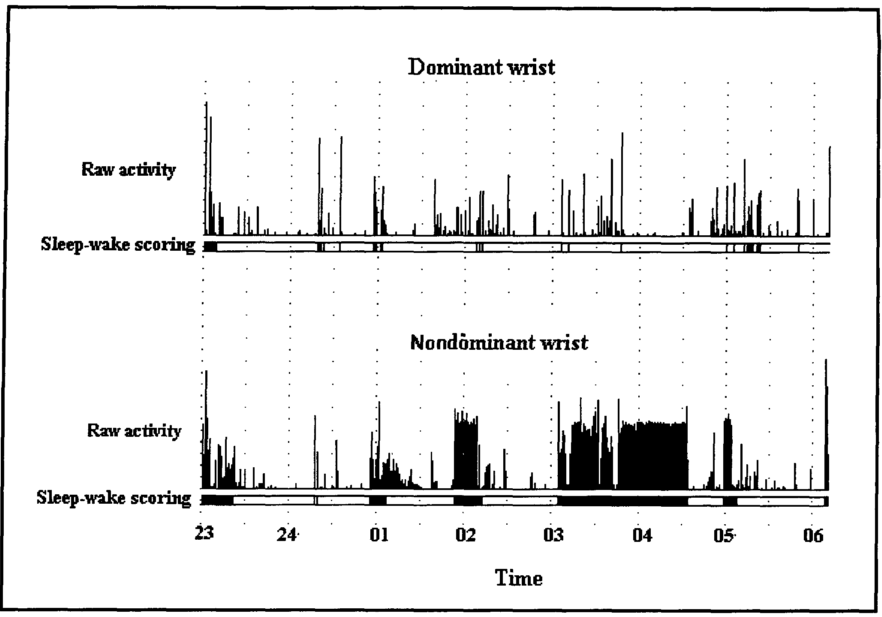
\includegraphics[scale=0.4]{Images/actiPlacement2.png}
\caption{Raw activity data and sleep-wake scoring from concommitant dominant and non-dominant wrist actigraphy (from~\cite{Sadeh1994})}
\label{actiPlacement2}
\end{figure}

\paragraph{}
In their study, Jean-Louis et al.~\cite{Jean-Louis1997a} placed an actigraph unit on the dominant wrist and another one on the dominant ankle. The participants wore the actigraph units for one night. The outputs of each actigraph were compared in order to find whether they were similar or strongly uncorrelated.

\paragraph{}
The study showed there was a strong correlation between the scoring using the activity from the actigraph unit placed on the wrist and the scoring using the activity from the ankle, as it can be seen on Fig.~\ref{actiPlacement1}.

\begin{figure}[H]
\centering
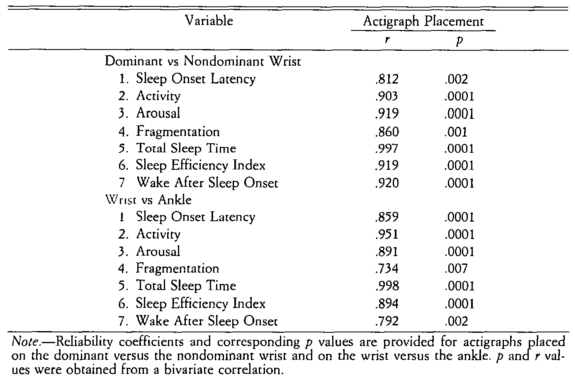
\includegraphics[scale=0.5]{Images/actiPlacement1.png}
\caption{Correlation between wrist and ankle placement of the actigraph unit (from~\cite{Jean-Louis1997a})}
\label{actiPlacement1}
\end{figure}

\paragraph{}
The same study was made by placing one unit on the dominant wrist and another one on the non-dominant wrist. The conclusion that was draw for this case was the same as for the wrist/ankle case: a correlation between the two signals exists and the placement has no significant influence on the sleep-wake scoring. Sadeh et al.~\cite{Sadeh1994} ran a similar study and came to the same conclusion.

\paragraph{}
The conclusion that can be drawn from these studies is that sleep-wake algorithms seem to be robust to the difference of activity from the divergent placements. \\
Thus, the placement of the actigraph is left to the will of the scientists running the studies. For example, if the participants are infants, it may be more convenient to place the actigraph on the ankle while, on the other hand, if the participants exhibits restless leg syndrome, the choice of the wrist seems more opportune.

\paragraph{}
An important point that must be kept in mind is that even though the algorithms are robust to the placement of the actigraph units, ''\textit{it is important to maintain
standard placement to minimize variability associated with actigraph location and to enable comparisons between individuals and between studies.}''~\cite{Sadeh2005}.

\paragraph{}
Finally, it may be relevant to use twin-wrist-actigraph units (one at each wrist) in order to avoid artifacts as the one seen one the Fig.~\ref{actiPlacement2}. This artifact is called a ''breathing artifact'' and resulted from placing the non-dominant wrist on the chest while sleeping. This led to appearance of activity while the subject was actually sleeping. When using the data from the dominant wrist, this artifact could easily be removed.\\
Of course, due to monetary and comfort constraints, it may not always be possible to use two actigraph units for all studies.

\subsubsection{Sensitivity after Extenstive Use}

\paragraph{}
This part of a study was done to establish whether the sensitivity of the actigraph units was altered after long-term use. The participants wore two actigraphs on the same (dominant) wrist: the new one that had never been used previously and the old one that had been used in other studies for at least eighteen months.

\paragraph{}
As it can be seen on the Fig.~\ref{actiReliability}, there is no significant changes in sensitivity over time. This means that old actigraph units\footnote{In this study, ''old'' means ''eighteen months old''} can still be used without a loss of precision in the results.

\begin{figure}[H]
\centering
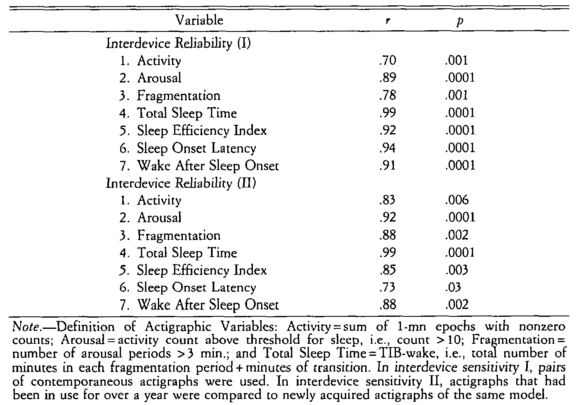
\includegraphics[scale=0.5]{Images/actiReliability.png}
\caption{Correlation between the old and new actigraph units outputs (from~\cite{Jean-Louis1997a})}
\label{actiReliability}
\end{figure}

\subsubsection{First Night Effect}

\paragraph{}
The first night effect ''\textit{refers to the influence a new setting (e.g., laboratory) may have on an individual's ability to sleep the first night away from home. Factors responsible for this observation include the unfamiliar setting which the sleep laboratory represents, the need to habituate oneself to wearing recording electrodes and to being monitored by others}''~\cite{Jean-Louis1997a}. If this effect impacts on the participants of actigraphy studies, it means that the first recorded night should always be dropped.

\paragraph{}
To assess whether this effect is significantly relevant in actigraphy studies, the participant of this part of the study wore an actigraph unit on the dominant wrist for at least three nights. If the first night was significantly different from the others, it would mean that the first night effect should be taken into account.

\paragraph{}
Jean-Louis et al. found ''\textit{no significant difference [...] for sleep duration between Night 1 and Night 2}''~\cite{Jean-Louis1997a}. This is illustrated on the Fig.~\ref{firstNightEffect}.

\begin{figure}[H]
\centering
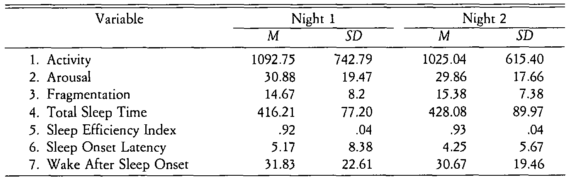
\includegraphics[scale=0.5]{Images/firstNightEffect.png}
\caption{Difference between first night and second night (from~\cite{Jean-Louis1997a})}
\label{firstNightEffect}
\end{figure}

\subsection{Recommendations}
\label{subsec:recommandations}
\paragraph{}
Lisa et al.~\cite{LisaJ.MeltzerHawleyE.Montgomery-DownsSalvatoreP.Insana2012} made a review of the ''\textit{research literature that used actigraphy as a measure of sleep-wake patterns or circadian rhythms among pediatric populations (ages 0–18 years, inclusive)}''. From that synthesis, they give recommandations about how to properly report results while performing actigraphy studies. They made the checklist that may be seen on the Fig.~\ref{checklistLisa}.

\begin{figure}[H]
\centering
\begin{tabularx}{\textwidth}{|X|c|}
\hline
& Check \\
\Ghline
\textbf{Device/System Information} & \\
$\bullet$ The name of the device, the specific model, and the name (and location) of the manufacturer & \\
\hline
$\bullet$ The placement of the device (non-dominant or dominant wrist, left or right ankle, etc.) & \\
\hline
$\bullet$ The measured epoch length, the mode of data collection (e.g., ZCM, TAT, PIM, or TRI), the use of the event marker, and the algorithm or wake sensitivity threshold & \\
\hline
$\bullet$ Justification for the algorithm that is chosen & \\
\hline
$\bullet$ The type and version of software used & \\
\hline
\textbf{Sleep Diary} & \\
$\bullet$ Type of sleep diary used (e.g., paper, electronic, telephone call) & \\
\hline
$\bullet$ Who completed sleep diary (i.e., parent, child) & \\
\hline
$\bullet$ Frequency of diary completion (e.g., at bedtime only, morning and evening) & \\
\hline
\textbf{Data Collection and Processing (including Missing Data)} & \\
\hline
$\bullet$ Number of nights of data collection & \\
\hline
$\bullet$ Number of weekday and weekend nights (if relevant) & \\
\hline
$\bullet$ Methods used to identify and handle artifact & \\
\hline
$\bullet$ How much data lost due to: & \\
$\;\; \bullet$ Technical failure & \\
$\; \bullet$ Participant non-adherence (to wearing the watch or completing the sleep diary) & \\
$\;\; \bullet$ Artifact & \\
\hline
\textbf{Data variables} & \\
\hline
$\bullet$ Clearly define the variables, including ones automatically calculated by manufacturer scoring programs (e.g., sleep bouts, wake bouts, motionless sleep or immobile time, circadian parameters) & \\
\hline
$\bullet$ Clearly define the scoring rules used, using common/standardized names & \\
\hline
\end{tabularx}
\caption{Proposed Standard Checklist for Reporting Actigraphy in Pediatric Sleep Research Literature (from~\cite{LisaJ.MeltzerHawleyE.Montgomery-DownsSalvatoreP.Insana2012})}
\label{checklistLisa}
\end{figure}

\paragraph{}
Berger et al.~\cite{Berger2008} made a similar study which gave the following checklist.

\begin{figure}[H]
\centering
\begin{tabularx}{\textwidth}{|X|c|}
\hline
& Check \\
\Ghline
\textbf{Instrumentation} & \\
\hline
$\bullet$ The word ‘‘actigraph’’ as a key word & \\
\hline
$\bullet$ Copyrighted or registered trademark name of the device, model, and name and location of the manufacturer & \\
\hline
$\bullet$ Placement of the actigraph (nondominant or dominant wrist/ankle) & \\
\hline
\textbf{Selection of pertinent variables} & \\
\hline
$\bullet$ Specific sleep, activity, and circadian rhythm variables & \\
\hline
$\bullet$ Clear definitions of selected variables & \\
\hline
\textbf{Sampling} & \\
\hline
$\bullet$ Data collection environment (home, hospital, or somewhere else) & \\
\hline
$\bullet$ Duration of data collection period & \\
\hline
$\bullet$ Number of sleep and activity intervals included (single/mean) & \\
\hline
$\bullet$ Days of the week (by name) & \\
\hline
$\bullet$ Sampling epoch length & \\
\hline
\textbf{Data processing and analysis} & \\
\hline
$\bullet$ Description of procedures used for preparing files & \\
\hline
$\bullet$ Description of decision rules made for setting time limits of entire file, setting time intervals, editing raw data, handling missing data, handling of naps prior to bedtime, etc. & \\
\hline
$\bullet$ Scoring reliability procedures and percent agreement & \\
\hline
$\bullet$ Name of software, mode, and algorithm used for scoring sleep & \\
\hline
\end{tabularx}
\caption{Actigraphy Information Suggested for Inclusion in Research Reports (from~\cite{Berger2008})}
\label{checklistBerger}
\end{figure}

\newpage

\section{State of the art}
\label{sec:stateOfTheArt}

\subsection{Webster's Algorithm}

Webster's algorithm~\cite{Webster1982} is one of the first algorithm developped for an automatic sleep/wake scoring system based on actigraphic data. Consequently, it is a method that can be qualified as ''basic'' as it doesn't involve any advanced processing method but only uses simple signal processing techniques.

\paragraph{}
They use an actigraph which gives an output values every 2 seconds. This choice comes from a compromises between the need for precision (Webster wanted to be able to identify if the patient was awake or asleep for every minute) and the limits of practicality.

\subsubsection{Method}

\paragraph{}
For every minute, a value is assigned to a variable $D$ based on a weighted sum of combinations of the actigraphic data:

\begin{equation}
\label{Webster_equationInit}
\begin{split}
SW = S * [&W(1)T(1) + W(2) T(2) + W(3) T(3) \\
         &+ W(4) T(4) + W(5) T(5) + W(6) T(6)]
\end{split}
\end{equation}

\paragraph{}
''\textit{where S is a scale factor; W is a weight; T(1) is the sum of the digital activity values for all 30 2-s data epochs in 1 min; T(2) is the activity value for the single most active epoch; T(3) is the sum of the activity values in the two most active epochs separated by at least 30 s; and T(4) is the sum of the activity values in the 8 most active epochs.}

\begin{equation}
T(5) = W(5, 1) T(i - 1) + W(5,2) T(i - 2) + W(5, 3) T(i - 3) + W(5, 4) T(i - 4)
\end{equation}
\begin{equation}
T(6) = W(6, 1) T(i + 1) + W(6, 2) T(i + 2)
\end{equation}

\paragraph{}
\textit{where T(i - 1) is the value of T(1) for the preceding minute, T(i + 1) for the following minute, etc.}''\cite{Webster1982}

\paragraph{}
Thus, for every minute, $D$ is computed and depending on its value, this minute is scored as ''sleep'' or ''wake'':

\begin{equation}
SW(n) = \left\{
    \begin{array}{ll}
        \mbox{wake} & \mbox{if } D \geq 1\\
        \mbox{sleep} & \mbox{otherwise}
    \end{array}
\right.
\end{equation}

\paragraph{}
The weights $W$ used in Eq.~\ref{Webster_equationInit} were then optimized in order to have the best agreement between the output of the algorithm $SW$ and the EEG sleep/wake score, used as a reference. As Webster et al. had 20 actigraphic records, they applied the optimization over 17 of them while keeping 3 of them as a ''control'' group that will be used to validate the results.

\paragraph{}
Once this optimization has been done, it appeared that the best agreement was obtained when $W(1) = W(3) = W(4) = 0$ which means that $T(1)$, $T(3)$ and $T(4)$ had no significant roles in the determination of $SW$.
This observation leaded to a new formulation of $D$:

\begin{equation}
\begin{split}
D = S * &[W(1) T(i-4) + W(2) T(i - 3) + W(3) T(i - 2)\\
         &+ W(4) T(i - 1) + W(5) T(i) + W(6) T(i+1) + W(7) T(i+2)]
\end{split}
\end{equation}

\paragraph{}
''\textit{Where Ws represent weights and TU) represents the maximal epoch value (T(2) in the previous expression) for the current minute, T(i - 1) for the previous minute, T(i + 1) for the succeeding minute, etc.}''\cite{Webster1982}

\paragraph{}
The weights were once again optimized to obtain the best agreement. This optimization gave this explicit definition of $D$:

\begin{equation}
\begin{split}
D = 0.025 * &[0.15 T(i-4) + 0.15 T(i - 3) + 0.15 T(i - 2)\\
         &+ 0.08 T(i - 1) + 0.21 T(i) + 0.12 T(i+1) + 0.13 T(i+2)]
\end{split}
\end{equation}

\paragraph{}
Even though the agreement between the output $SW$ and the EEG score was already quite good (see \ref{subsubsec:websterResults}), some additional rules were applied to $SW$ to achieve an even better agreement.

\begin{itemize}
\item after at least 4 min scored wake, the first period of 1 min scored sleep is rescored wake;
\item after at least 10 min scored wake, the first 3 min scored sleep are rescored wake;
\item after at least 15 min scored wake, the first 4 min scored sleep are rescored wake;
\item 6 min or less scored sleep surrounded by at least 10 min (before and after) scored wake are rescored wake;
\item 10 min or less scored sleep surrounded by at least 20 min (before and after) scored wake are rescored wake.
\end{itemize}

\subsubsection{Results}
\label{subsubsec:websterResults}

\paragraph{}
By applying the first version of their algorithm (without the additional conditions), Webster et al. achieve an overall agreement of the 17 records used for the optimization of 94.46\%. The agreement of the 3 records that were not used was 96.02\%.

\paragraph{}
A more detailed analysis of these results showed that ''\textit{the conditional probability of misscoring wake as sleep was higher (.062) than misscoring sleep as wake (.039)}''\cite{Webster1982}. Two elements are the main reason of this difference:

\begin{itemize}
\item While the patient is awake, he may have some short periods of inactivity. The opposite (short periods of activity during the night) is less frequent.
\item There is a delay (called ''sleep onset'') between the time when all activity ceases and the time when the patient effectively falls asleep
\end{itemize}

\paragraph{}
This is the reason why the additional rules were added. They lead to better agreements: 94.74\% for the 17 records used at the optimization step (previously: 94.46 \%). No results are presented for the 3 last records.
More importantly, these new rules lead to a drop of the overestimation of the proportion of sleep from the algorithm compared to the EEG from 1.89\% to 0.81\%.

\subsection{Sadeh's Algorithm}
\label{subsec:sadeh}

\subsubsection{Method}

\paragraph{}
3 states are defined by Sadeh et al. \cite{Sadeh1995} : wake, active sleep and quiet sleep. \\

To determine the patient's state at each period, some parameters are defined :
\begin{quotation}
\em 
\item ''\textbf{nzm} : number of minutes with zero activity in the global window (the scored minute plus the 5 min that precede it and follow it);
\item \textbf{ntl} : number of minutes with low activity (nonzero but lower than 100 counts) in the global window;
\item \textbf{nth} : number of minutes with high activity (equal or greater than 100 counts) in the global window;
\item \textbf{s}$_5$ : standard deviation of the window of the scored minutes plus the 5 min preceding it;
\item \textbf{m}$_1$ : mean activity level of the scored minute and the preceding minute;
\item \textbf{lw}$_4$ : the lowest activity count during the window that includes the scored minute plus the following 4 min. ''~\cite{Sadeh1995} 
\end{quotation}

\paragraph{}
The probabilities of each state are defined as :

\begin{equation}
\begin{split}
PQS =& 15.94 + 3.223\: nzw + 2.138\: ntl + 1.1036\: nth \\
      &+ 0.0466\: s_5 + 0.00292\: m_1 + 0.0106\: lw_4
\end{split}
\end{equation}

\begin{equation}
\begin{split}
PAS =& 5.134 + 1.696\: nzw + 2.062\: ntl + 0.9568\: nth \\
      &+ 0.0585\: s_5 + 0.00556\: m_1 + 0.0105\: lw_4
\end{split}
\end{equation}

\begin{equation}
\begin{split}
PAW =& -25.638 + 1.714\: nzw + 3.0168\: ntl + 4.064\: nth \\
      &+ 0.1066\: s_5 + 0.0386\: m_1 + 0.016\: lw_4
\end{split}
\end{equation}

where $PQS$ is the probability to be in the quiet sleep state, $PAS$ in the active sleep state and $PAW$ in the wake state.

\paragraph{}
For every minute of the recorded signal, $PQS$, $PAS$ and $PAW$ are computed and the state of the patient is determined by the greatest of these three values.

\subsubsection{Results}

\begin{figure}[H]
\centering
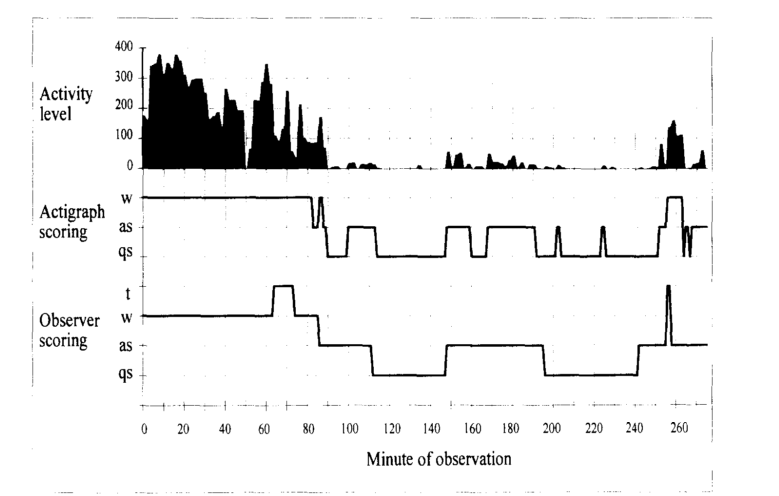
\includegraphics[scale=0.5]{Images/SadehResults1.png}
\caption{Minute-by-minute correspondence of the raw activity data with the resulting actigraphic scoring and the observer's state scoring in a 3-month-old infant. QS = quite sleep; AS = active sleep; W = wake; T = transition or uncertain period. (from~\cite{Sadeh1995})}
\label{SadehResults1}
\end{figure}

\paragraph{}
Sadeh et al.~\cite{Sadeh1995} obtained an agreement rate of $93.5\%$ for wakefulness, of $74.9\%$ for active sleep and of $78.0\%$ for quiet sleep. This leads to an agreement rate for sleep-wake states of $95.6\%$. \\
They noticed that the transition epochs (from wake to sleep or sleep to wake) were usually scored as active sleep ($68.6\%$) or wake ($31.4\%$) but rarely as quiet sleep.

\subsection{Pires' Algorithm}

\paragraph{}
Pires algorithm \cite{Pires2009} is based on the observation that the actigraphic signal consists of a combination of two main components: one that is more dominant during the day and the other one that is more dominant during the night. Therefore, the output signal of the algorithm is a mix of two distributions which model these two components. Depending on which distribution is prevalent at each time n, the algorithm will decide whether the patient is awake or asleep.

\subsubsection{Method}

\paragraph{}
The first distribution must model the main component during daytime and is noted $p_d(r)$. As the movements during daytime are usually purposeful, the distribution used to model the actigraph output during daytime must copy this purposefulness. Pires makes the assumption that the three accelerations are independent and identically non zero mean Gaussian distributed: $p(a_x) = p(a_y) = p(a_z) = \mathcal{N}(\mu, \sigma^2)$. Given this, the acceleration magnitude ($r = \sqrt{a_x^2 + a_y^2 + a_z^2}$) is modeled as a shifted Maxwell distribution $\mathcal{M}(c_\mathcal{M}, \sigma_\mathcal{M})$:

\begin{equation}
p_d(r) = \sqrt{\frac{2}{\pi}} \frac{(r - c_{\mathcal{M}})^2}{\sigma_{\mathcal{M}}^3} e^{-\frac{(r - c_{\mathcal{M}})^2}{\sigma_{\mathcal{M}}^2}}
\end{equation}

\paragraph{}
This distribution arises if the three accelerations are truly independent and identically non zero mean Gaussian distributed.

\paragraph{}
The second distribution must model the main component during nighttime and will be noted $p_n(r)$. Contrary to what happens during daytime, the movements during nighttime are usually purposeless and non coherent. This is why the acceleration magnitude during nighttime is modeled as a Poisson distribution (but in the paper, a Gaussian distribution is used for the sake of simplicity) $\mathcal{N}(c_\mathcal{N}, \sigma_\mathcal{N}^2)$:

\begin{equation}
p_n(r) = \frac{1}{\sqrt{2\pi}} \frac{1}{\sigma_\mathcal{N}} e^{-\frac{(r - c_{\mathcal{N}})^2}{2\sigma_{\mathcal{N}}^2}}
\end{equation}

\paragraph{}
The output signal is then modeled as a combination of these two distributions:

\begin{equation}
\label{PiresProb}
\begin{split}
p(r, \theta) & = \alpha p_d(r) + \beta p_n(r) \\
 & = \alpha \sqrt{\frac{2}{\pi}} \frac{(r - c_{\mathcal{M}})^2}{\sigma_{\mathcal{M}}^3} e^{-\frac{(r - c_{\mathcal{M}})^2}{\sigma_{\mathcal{M}}^2}} + \beta \frac{1}{\sqrt{2\pi}} \frac{1}{\sigma_\mathcal{N}} e^{-\frac{(r - c_{\mathcal{N}})^2}{2\sigma_{\mathcal{N}}^2}}
\end{split}
\end{equation}

\paragraph{}
where $\theta(n) = \{\underbrace{\alpha(n), \sigma_\mathcal{M}(n), c_\mathcal{M}(n)}_{\theta_\mathcal{M}(n)}, \underbrace{\beta(n), \sigma_\mathcal{N}(n), c_\mathcal{N}(n)}_{\theta_\mathcal{N}(n)} \}^T$ is estimated at each discrete time n.

\begin{figure}[H]
\centering
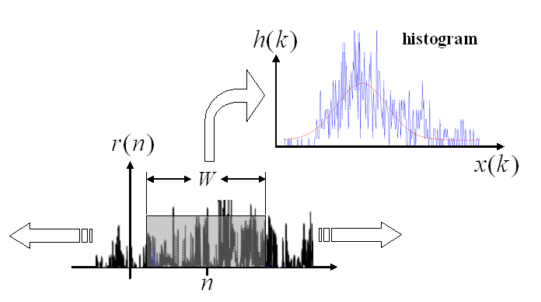
\includegraphics[scale=0.5]{Images/PiresActivity.png}
\caption{Windowing parameter estimation with histogramm fitting (from \cite{Pires2009})}
\label{PiresActivity}
\end{figure}

\paragraph{}
''\textit{The estimation of $\theta(n)$ at each instant n is performed by solving the following equation}

\begin{equation}
\theta(n) = \operatornamewithlimits{argmin}\limits_{\theta} \sum_{k=1}^L (h_n(k) - p(x_k, \theta))^2
\end{equation}

\paragraph{}
\textit{where $0 < n \leq N$, $\mathbf{h}_n = \{h_n(1), \ldots, h_n(L)\}$ is the L dimensional histogram with bins centered at locations $\mathbf{x} = \{x_1, x_2, \ldots, x_L\}$ computed in a W dimensional window centered at the $n^{th}$ sample and $p(x_k, \theta)$ is the function \ref{PiresProb} computed at locations $x_k$ as shown in Fig.\ref{PiresActivity}}.''\cite{Pires2009}

\paragraph{}
The signal $\theta(n)$ gives a more accurate representation of the activity than the raw acceleration magnitude. By observing the values of the parameters $\alpha(n)$ and $\beta(n)$ along the circadian cycle, the relative importance of each distribution may be obtained. During the day, $p_d(n)$ is prevalent while $p_n(n)$ is prevalent during the night.

\paragraph{}
Now that we have a more complete and accurate representation of the activity, the sleep/wakefulness state of the patient may be obtained. The sleep/wakefulness state a each time $n$ is defined as follows :

\begin{equation}
SW(n) = \left\{
    \begin{array}{ll}
        0 & \mbox{if sleep} \\
        1 & \mbox{otherwise}
    \end{array}
\right.
\end{equation}

\paragraph{}
First, to obtain this output signal, the difference $sw(n)$ is computed :

\begin{equation}
sw(n) = \alpha(n) - \beta(n)
\end{equation}

\paragraph{}
where $\alpha(n)$ and $\beta(n)$ are the parameters defined above. Thus, $sw(n)$ gives the preponderant distribution at each time n. If $p_d(n)$ is preponderant, $\alpha(n)$ is greater than $\beta(n)$ and $sw(n) > 0$. If $p_n(n)$ is preponderant, $\beta(n)$ is greater than $\alpha(n)$ and $sw(n) < 0$.

\paragraph{}
$SW(n)$ is then estimated from the signal $sw(n)$ :

\begin{equation}
\hat{\mathbf{SW}}(n) = \operatornamewithlimits{argmin}\limits_{\mathbf{SW}} E(\mathbf{sw}, \mathbf{SW})
\end{equation}

\paragraph{}
where $\mathbf{SW} = \{SW(1), SW(2), \ldots, SW(N) \}^T$, $\mathbf{sw} = \{sw(1), sw(2), \ldots, sw(N) \}^T$ and

\begin{equation}
E(\mathbf{sw}, \mathbf{SW}) = \underbrace{\sum_n sw(n) (1 - 2SW(n))}_{\mbox{binarization}} + \underbrace{\gamma \sum_n |SW(n) - SW(n-1)|}_{\mbox{regularization}}
\end{equation}

\paragraph{}
The binarization term forces $sw(n)$ to observe the following rule

\begin{equation}
SW(n) = \left\{
    \begin{array}{ll}
        0 & \mbox{if} sw(n) < 0 \\
        1 & \mbox{otherwise}
    \end{array}
\right.
\end{equation}

\paragraph{}
The regularization term forces a ''\textit{stepwise constant solution with abrupt transitions by introducing temporal correlation between neighboring samples, $|SW(n) - SW(n-1)|$, where differences between consecutive samples of SW are penalized by}''\cite{Pires2009} $\gamma$. A greater $\gamma$ leads to a greater penalization and therefore a more stepwise constant solution whereas a smaller $\gamma$ leads to the opposite. The parameter $\gamma$ is manually chosen to obtain an output signal that is not (too much) affected by the noise from $sw(n)$ but that is still related to the genuine transitions coming from the changes of state of the patient.

\subsubsection{Results}

\begin{figure}[H]
\centering
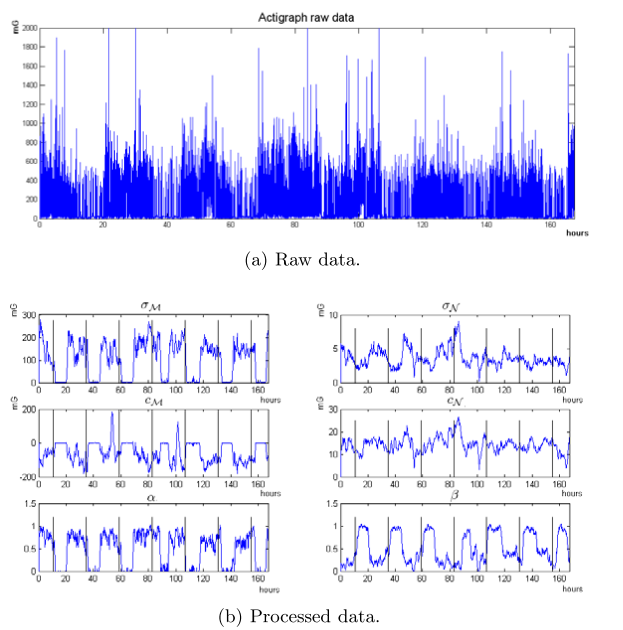
\includegraphics[scale=0.5]{Images/PiresResults1.png}
\caption{Real example acquired during 167 hours (from~\cite{Pires2009})}
\label{PiresResults1}
\end{figure}

\begin{figure}[H]
\centering
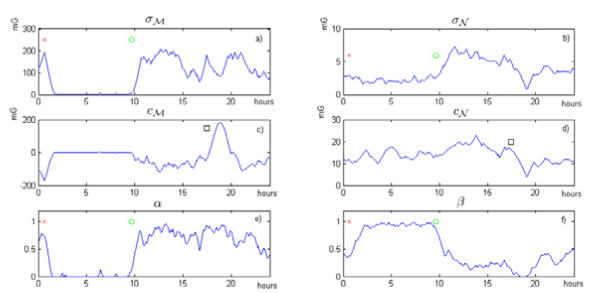
\includegraphics[scale=0.5]{Images/PiresResults2.png}
\caption{Zoom from Fig.~\ref{PiresResults1}. The ''x'' and ''o'' marks indicate the ''go to bed'' and the ''get out of bed'' events(from~\cite{Pires2009})}
\label{PiresResults2}
\end{figure}

\begin{figure}[H]
\centering
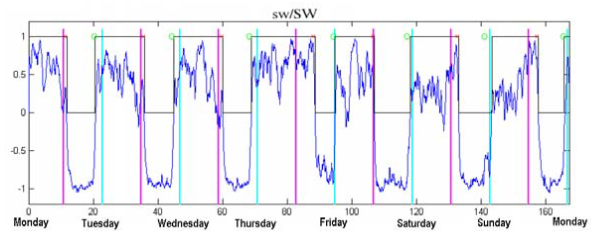
\includegraphics[scale=0.5]{Images/PiresResults3.png}
\caption{Representation of the Sleep/Wakefulness (SW) state. Vertical magenta lines represent the midnight instants and the cyan ones represent the midday. ''x'' and ''o'' marks indicate the ''go to bed'' and the ''get out of bed'' events. The dark binary signal represents $SW(n)$, the blue signal represents $sw(n)$ (from~\cite{Pires2009})}
\end{figure}

\paragraph{}
The first element that may be noticed from these results is that the signal $\alpha(n) + \beta(n)$ is approximately 1 (mean = 0.98, standard deviation = 0.096) which means that the mixture of $p_d(n)$ and $p_n(n)$ gives a good estimation of the real actigraphic signal.

\paragraph{}
Secondly, it is clear that between the ''go to bed'' and the ''get out of bed'' events (during the night), $\beta$ is greater than $\alpha$, which is really close to zero. That means that the Poisson distribution $p_n(n)$ is indeed prevalent during the night. Conversely, during the dat, the Maxwell distribution $p_d(n)$ is dominant.

\paragraph{}
Even though the results \textit{looks} quite accurate, Pires et al. only show the application of their algorithm on one patient. They also do not provide any statistical detail such as the error rate, the sensitivity, the specificity, etc. which makes it difficult to know how well their method works. \\
Finally, no information about the patient (their age, are they healthy ?, ...) are given.

\subsection{Crespo's Algorithm}

\paragraph{}
Crespo's Algorithm\cite{Crespo2012} is composed of two main stages. The first one is called the 'preprocessing stage' and produces an estimate of the sleep-wake periods. The second one is the 'processing and decision stage'. This stage uses the output of the preprocessing stage and produces the final identitification of the sleep-wake periods.

\paragraph{}
The signal from the actigraph is denoted as $s(n)$, or as $\mathbf{s} = (s_1, s_2, ..., s_N)$ where $N$ is the number of elements in $\mathbf{s}$ (i.e. the number of measures available). The sampling rate for all the actigraphs used by Crespo et al. is one sample per minute.

\paragraph{}
All the equations in the section come from \cite{Crespo2012}.

\subsubsection{Preprocessing stage}
\label{subsubsec:preprocessing}
\paragraph{Signal conditioning based on empirical probability model\\}
Firstly, a function $F\{.\}$ is applied to $s(n)$ in order to determine the regions containing more than $\zeta$ consecutives zeroes. The indexes of these zeros are then put in the vector $\mathbf{a}$.

\begin{equation}
\mathbf{a} = F\{s(n), \zeta\}
\end{equation}

\paragraph{}
Secondly, all the $s(i)$ where $i$ is contained in $\mathbf{a}$ are replaced by the value $s_t$ where $s_t$ is the $t^{th}$percentile of s(n). The new signal obtained is then stored in $x(n)$.

\begin{equation}
x(j) = \left\{
    \begin{array}{ll}
        s_t & \mbox{if } j \in \mathbf{a} \\
        s(j) & \mbox{if } j \notin \mathbf{a}
    \end{array}
\right.
\end{equation}

Before applying a median operator to $x(n)$, the signal is padded, in order to facilitate this filtering. 

\begin{equation}
\label{padding}
x_p = (\underbrace{m, m, \ldots, m}_{30 * \alpha}, x_1, x_2, \ldots, x_N, \underbrace{m, m, \ldots, m}_{30 * \alpha})
\end{equation}

\paragraph{}
$(30 * \alpha)$ elements are added at the begining and the end of $x(n)$. All these elements have the same value which is $m = max(s(n))$. $\alpha$ is a paramater that can be modified to optimize the algorithm. It is used to define the window length of the median filtering, $L_w = (60 * \alpha + 1)$ and it represents the length of the window in hours. \\

Depending on the value of $\alpha$, the determination of the sleep-wake periods will be more or less accurate. A large $\alpha$ gives the right number of transitions while a small $\alpha$ gives a more precise time for these transitions. The value of $\alpha$ is determined as a tradeoff between these two properties of the result.


\paragraph{Rank-order processing and decision logic\\}
Now that the signal is padded, the median operator $M\{.\}$ may be applied.

\begin{equation}
\begin{split}
x_f(n) = & M\{x_p(n - 30 * \alpha), x_p(n - 30 * \alpha + 1), \ldots,\\
         & x_p(n - 1), x_p(n), x_p(n+1), \ldots, x_p(n + 30 * \alpha)\}
\end{split}
\end{equation}

\paragraph{}
\label{T-threshold}
The obtained signal $x_f(n)$ is filtered by a rank-order thresholding operator $T\{.\}$.

\begin{equation}
y_1(n) = T\{x_f(n)\} = \left\{
    \begin{array}{ll}
        1 & \mbox{if } x_f(n) > p \\
        0 & \mbox{otherwise}
    \end{array}
\right.
\end{equation}

where the threshold $p$ is the percentile of $x_f(n)$ corresponding to $\frac{h_s}{24}*100\%$. $h_s$ is the average duration of sleep per night (in hours).

\paragraph{Morphological filtering}
\label{closing-opening}
Finally, the signal is filtered by a morphological closing followed by a morphological opening. Explanations about morphological operations may be found in the Annex \ref{sec:morphology}.

This operation leads to the deletion of incorrect transitions (i.e. transitions that are too short)

\begin{equation}
y_e(n) = (y_1(n) \bullet L_p) \circ L_p
\end{equation}

where $L_p$ is the length of the window in minutes.

\paragraph{}
$y_e(n)$ is the output of the preprocessing stage. It is a rough estimator of the sleep-wake periods and will be used in the processing stage to get a more refined model.

\subsubsection{Processing}

\paragraph{Model-based data validation}
A function $G\{.\}$ is applied to the original signal $s(n)$ in order to determine the regions containing more than $\zeta^r$ consecutives zeroes during estimated rest periods and more than $\zeta^a$ consecutives zeroes during estimated wake periods. The indexes of these zeros are then put in the vector $\mathbf{b}$.

\begin{equation}
\mathbf{b} = G\{s(n), \zeta^r, \zeta^a\}
\end{equation}

\paragraph{Adaptive rank-order processing and decision logic}
As done in the preprocessing stage, the signal is padded to facilitate the filtering that comes next. 60 elements are added at the begining and the end of $s(n)$. All these elements have the same value which is $m = max(s(n))$.

\begin{equation}
x_{sp} = (\underbrace{m, m, \ldots, m}_{60}, s_1, s_2, \ldots, s_N, \underbrace{m, m, \ldots, m}_{60})
\end{equation}

\paragraph{}
The adaptive median filter $M_a\{.\}$ with a varying window length is then applied on $x_{sp}$. The output $x_{fa}(i)$ of this filter is the median of the values of $x_{sp}(n)$ in the window centered about $i$, that are not contained in $\mathbf{b}$.
The window begins with a length of one hour and it increases until it reaches the maximum length $L_w$.

\begin{equation}
x_{fa} = M_a\{x_{sp}(n), \mathbf{b}, L_w\}
\end{equation}

\paragraph{}
The next step is a thresholding by the rank-order operator $T\{.\}$ defined in the preprocessing stage (\ref{T-threshold})

\begin{equation}
y_2(n) = T\{x_{fa}(n)\} = \left\{
    \begin{array}{ll}
        1 & \mbox{if } x_{fa}(n) > p \\
        0 & \mbox{otherwise}
    \end{array}
\right.\end{equation}

\paragraph{Morphological filtering}
The last step of the processing stage is the morphological filtering of $y_2(n)$ by a closing-opening, like done at the end of the preprocessing stage (\ref{closing-opening}). The difference here is that the window length $L_p'$ is double in size to $L_p$ : $L_p' = 2 * (L_p - 1) + 1$.

\begin{equation}
o(n) = (y_1(n) \bullet L_p') \circ L_p'
\end{equation}

\paragraph{}
$o(n)$ is the final output of the algorithm. It has a value for each period of the signal. An awake state is represented by a 1 while a rest state is represented by a 0.

%\subsection{Srinivasan method}
%
%\paragraph{}
%Srinivasan et al.~\cite{Srinivasan2010} ran a study slightly different from the other ones presented above. Their goal was to recognize real-life activities (called ADL - Activities of Daily Living) from actigraphic data. Not only did they want to distinguish wake from sleep but they also wanted to recognize which activity the participants were doing at each time of the day.
%
%\paragraph{}
%The fundation of their work was that actigraphy patterns differ depending on which activity is done, as it can be seen on the Fig.~\ref{activityPatterns}.
%
%\begin{figure}[H]
%\centering
%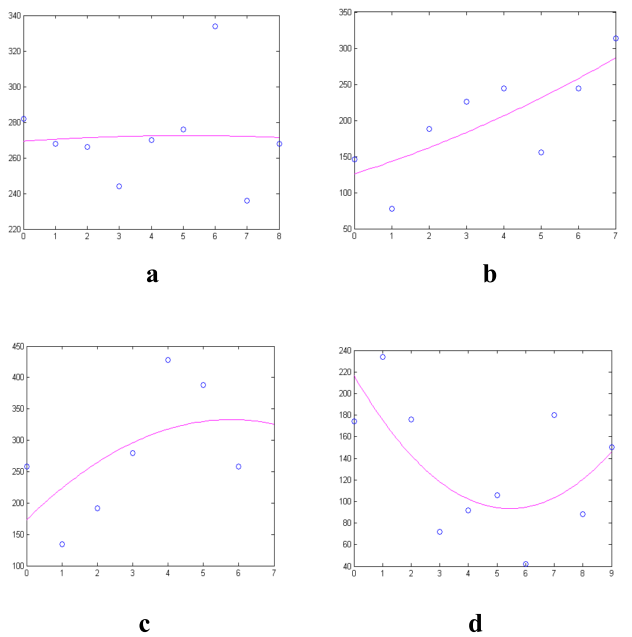
\includegraphics[scale=0.5]{Images/activityPatterns.png}
%\caption{Figure 2. Curve fitting using a least-square method of ADLs for ZC values. (a. Cooking; b. Eating; c. Hygiene; d. Watching Movie) (from~\cite{Srinivasan2010})}
%\label{activityPatterns}
%\end{figure}
%
%\paragraph{}
%In addition to the actigraphic data, the scientists also had information on when which activity was done. As the raw actigraphic data (ZC values) are not enough and cannot be easily used to predict activities, they extracted some additional features from the dataset that will be more helpful for the prediction:
%
%\begin{quotation}
%\em 
%\item ''\textbf{Min ZC Value:} the minimum zero-crossing value of an activity. This value is calculated for every instant of the activity
%\item \textbf{Max ZC Value:} the maximum zero-crossing value of an activity for every instant of the activity
%\item \textbf{Sleep Status:} the sleep/awake status of the participant. This value is generated through the Actigraph software after extracting the raw data
%\item \textbf{Time Length:} the amount of time taken for the completion of an activity. This value is calculated for every instant of the activity
%\item \textbf{Begin Hour:} the time of day is split into a 24 parts with each part denoting an hour. The begin hour of every activity is calculated for each occurrence of the activity
%\item \textbf{Number of events:} the total number of actigraph events per activity calculated for every instance
%\item \textbf{Bin:} we discretized the raw ZC value data into five interval sizes by equal width binning
%\item \textbf{Total ZC Value:} the total ZC value obtained for each activity for every instant
%\item \textbf{Pre-Activity:} we note every activity’s previous activity
%\item \textbf{Post-Activity:} the following activity of every activity is taken as the post activity''~\cite{Srinivasan2010}
%\end{quotation}

\newpage

\section{Our algorithm}
\label{method}
\subsection{Preprocessing stage}
\paragraph{}
The preprocessing stage is necessary standardize the actigraphic signals. As shown below (fig. \ref{preprocessing}), some input signals are not directly usable. Sometimes, the actigraph was switched on days before the subject began to wear it (fig. \ref{tooSoon}). Sometimes, the subject removed it during the day to carry out a task (having a wash, doing some sports, ...) (fig. \ref{tasks}).

\begin{figure}[H]
\centering
\subfigure[Too early turning on]{
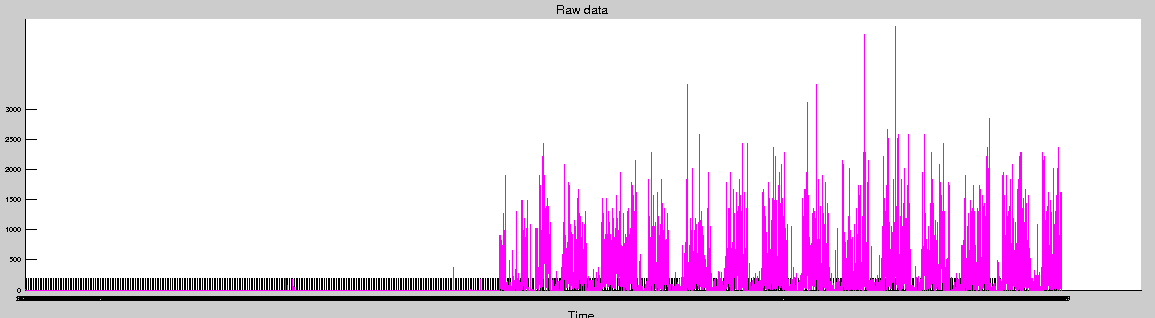
\includegraphics[scale=0.25]{Images/tooSoon.png}
\label{tooSoon}}
\subfigure[Actigraph unit removed]{
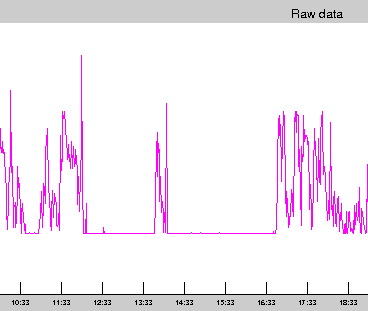
\includegraphics[width=10cm,height=4cm]{Images/tasks.png}
\label{tasks}}
\caption{Example of ''bad'' actigraphic data}
\label{preprocessing}
\end{figure}

\paragraph{}
In the first case, the "useless" beginning part is removed. This is done by using a sliding window along the signal. A count of the activities above a certain threshold in the window is made. If this count is greater that $\frac{3}{4}$ the size of the window, it is assumed that the subject has begun wearing the actigraph. All the values before this point are then simply removed from the signal.

\paragraph{}
The second case is trickier as the periods where the actigraph is removed may be mistaken for sleep periods. An observation of these two periods shows that the signal is completly non-existent while the actigraph is removed whereas it still has sporadic activities during the sleep periods. Then, in order to distinguish between the two options, a method similar to the one used for the first case is used again. \\
A window slides along the signal. A count of the activities in the window is made. If this count is lower that $\frac{1}{10}$ the size of the window, it is assumed that the subject has removed the actigraph and all the values inside the window are set to the maximum value of the entire signal.

\subsection{Processing stage}
\label{subsec:processing}
\paragraph{}
The aim of the preprocessing stage is to achieve a rough estimate of the sleep-wake periods. It must provide the correct number of transitions but the times when these transitions happens does not need extreme precision. This goal fits the preprocessing stage (\ref{subsubsec:preprocessing}) of the Crespo algorithm.

\paragraph{}
The motivations behind this choice are multiple:

\begin{itemize}
\item According to Crespo et al.~\cite{Crespo2012}, their algorithm was more performant when compared to other (older) methods
\item Indeed, when tested it was the method that gave the best results
\item It does not require ''optimized parameters''. Most of the parameters used have a physical sense. For instance, $h_s = 8h$ because it is estimated that an healthy person sleeps for about 8h per night. Other algorithms (such as Sadeh's Algorithm~\ref{subsec:sadeh}) use parameters that are optimized by the data and have no physical meaning. Therefore, it is hard to assess wether these techniques would work on other data sets and, theoretically with other actigraph units.
\end{itemize}

%Réexpliquer l'algorithme de Crespo + donner les valeurs de alpha, Lp, etc.

\paragraph{}
As a reminder, a summarised presentation of the preprocessing stage of Crespo's algorithm is given below, as well as the values of the parameters used. Along with this explanation, figures of the signal at different steps of the stage are given to give a practical insight of the action of each step.

\paragraph{Signal conditioning based on empirical probability model\\}
The first step of the preprocessing stage of Crespo's algorithm was not applied in our method. Its use was to remove consecutive zeros periods that were ''too long''. As this work is already done in our own preprocessing stage (see Fig.~\ref{tasks}), there was no use in doing it again in this stage.

\paragraph{Rank-order processing and decision logic\\}
Before applying a median operator to $x(n)$ (here, $x(n) = ACTI_{pre\_processed}(n)$, the signal is padded, in order to facilitate this filtering. 

\begin{equation}
\label{padding}
x_p = (\underbrace{m, m, \ldots, m}_{30 * \alpha}, x_1, x_2, \ldots, x_N, \underbrace{m, m, \ldots, m}_{30 * \alpha})
\end{equation}

Now that the signal is padded, the median operator $M\{.\}$ may be applied.

\begin{equation}
\begin{split}
x_f(n) = & M\{x_p(n - 30 * \alpha), x_p(n - 30 * \alpha + 1), \ldots,\\
         & x_p(n - 1), x_p(n), x_p(n+1), \ldots, x_p(n + 30 * \alpha)\}
\end{split}
\end{equation}

\begin{figure}[H]
\centering
\subfigure[Raw activity]{
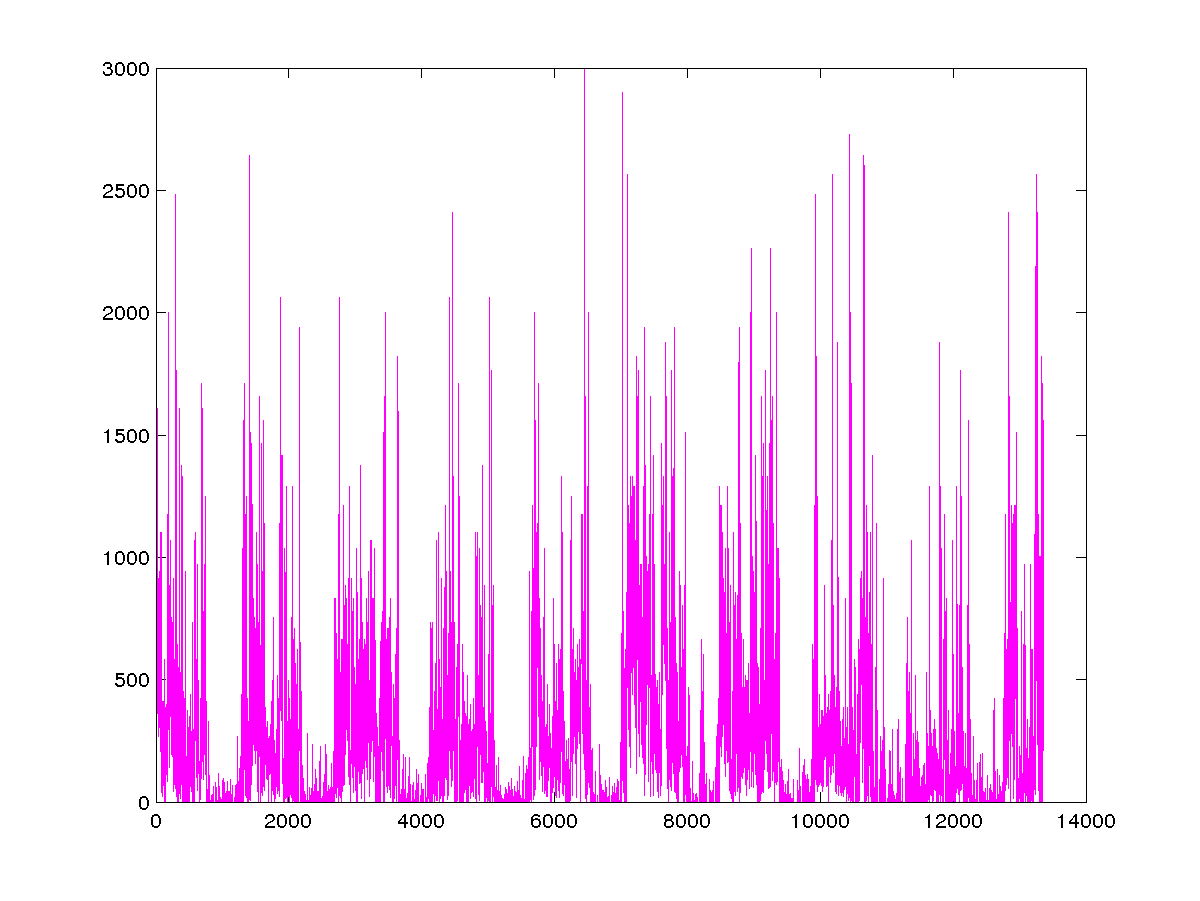
\includegraphics[scale=0.5]{Images/raw.png}}
\subfigure[$x_f(n)$]{
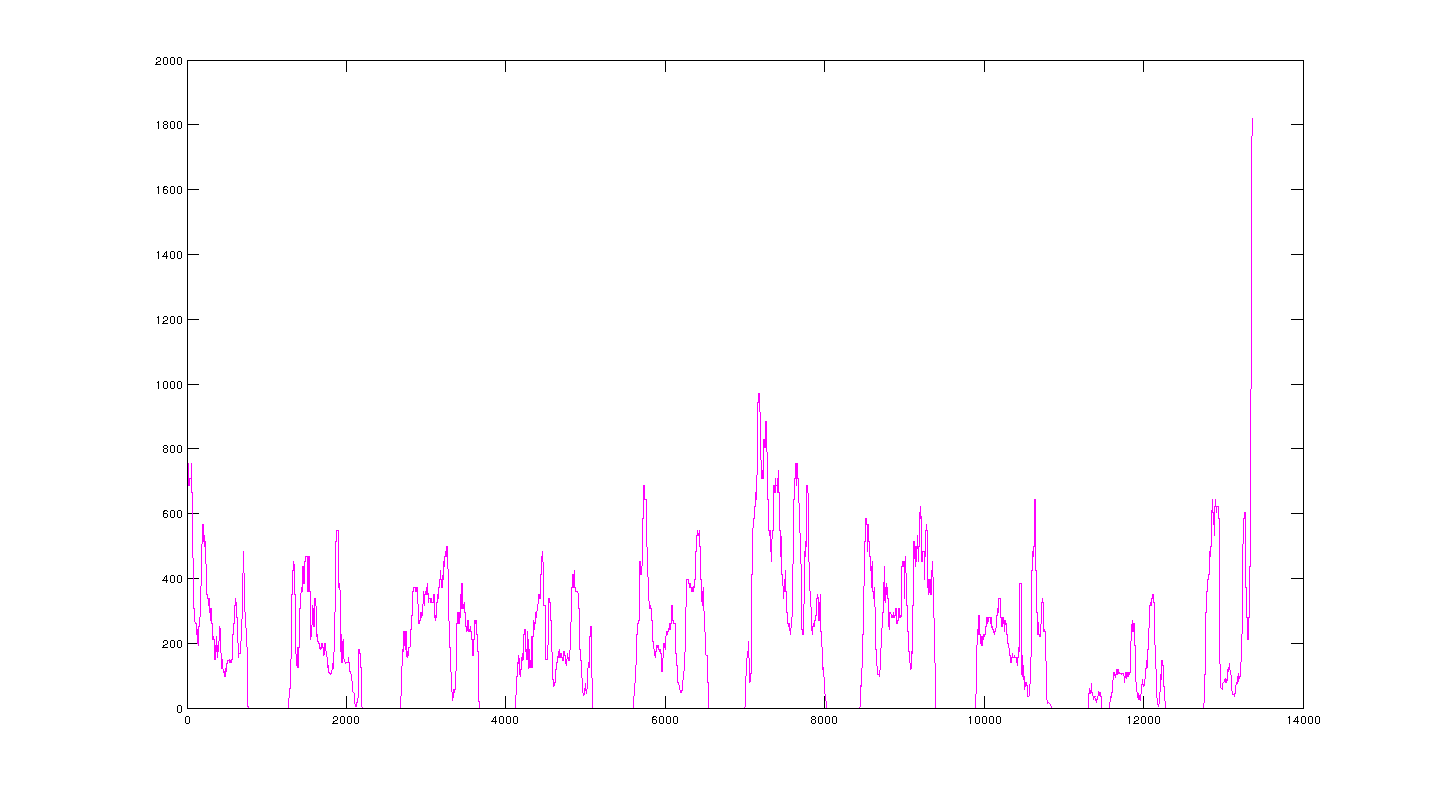
\includegraphics[scale=0.25]{Images/median.png}}
\caption{Illustration of the median filtering}
\end{figure}

\paragraph{}
\label{T-threshold}
The obtained signal $x_f(n)$ is filtered by a rank-order thresholding operator $T\{.\}$.

\begin{equation}
y_1(n) = T\{x_f(n)\} = \left\{
    \begin{array}{ll}
        1 & \mbox{if } x_f(n) > p \\
        0 & \mbox{otherwise}
    \end{array}
\right.
\end{equation}

where the threshold $p$ is the percentile of $x_f(n)$ corresponding to $\frac{h_s}{24}*100\%$. $h_s$ is the average duration of sleep per night (in hours).

\begin{figure}[H]
\centering
\subfigure[Raw activity]{
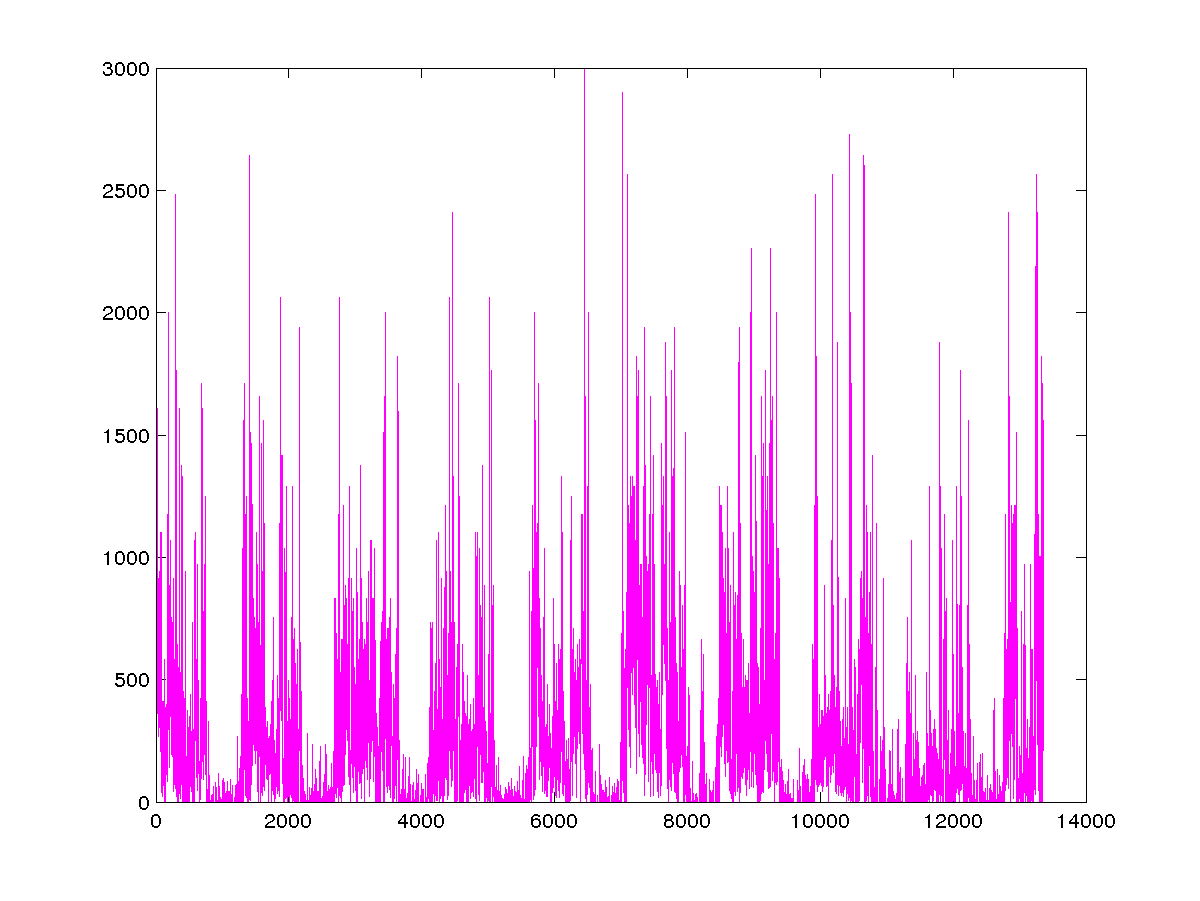
\includegraphics[scale=0.5]{Images/raw.png}}
\subfigure[$y_1(n)$]{
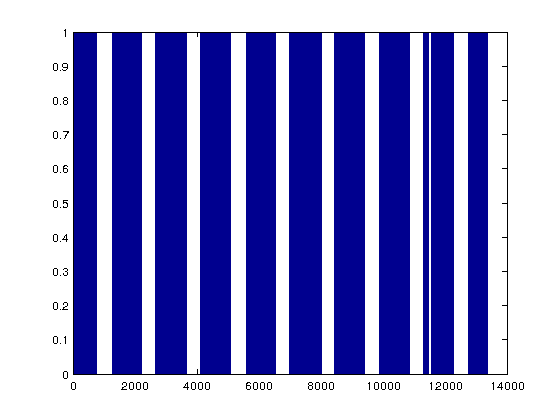
\includegraphics[scale=0.5]{Images/rankOrder.png}}
\caption{Illustration of the rank order filtering}
\end{figure}

\paragraph{Morphological filtering}
\label{closing-opening}
Finally, the signal is filtered by a morphological closing followed by a morphological opening. This operation leads to the deletion of incorrect transitions (i.e. transitions that are too short)

\begin{equation}
y_e(n) = (y_1(n) \bullet L_p) \circ L_p
\end{equation}

where $L_p$ is the length of the window in minutes.

\paragraph{}
$y_e(n)$ is the output of the preprocessing stage. It is a rough estimator of the sleep-wake periods and will be used in the next stage to get a more refined model.

\begin{figure}[H]
\centering
\subfigure[Raw activity]{
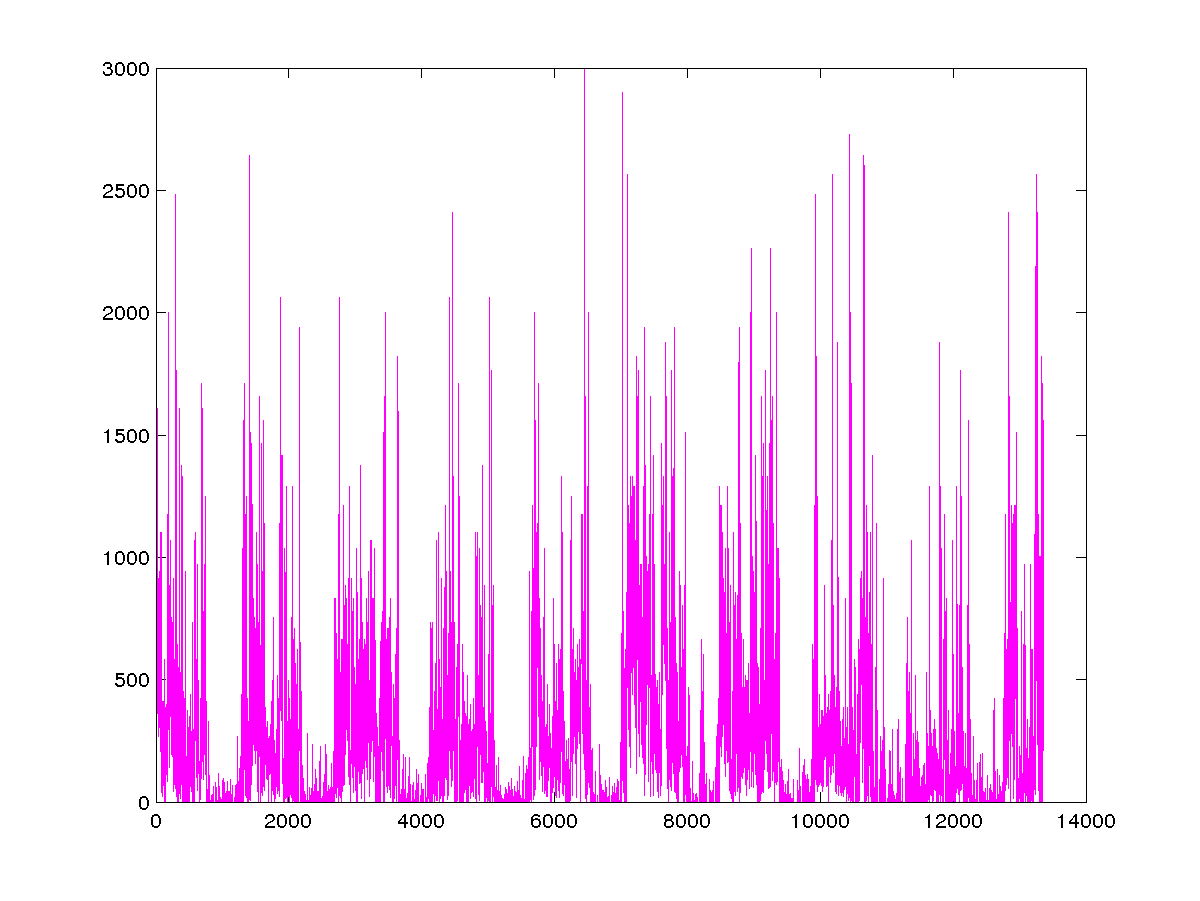
\includegraphics[scale=0.5]{Images/raw.png}}
\subfigure[$y_e(n)$]{
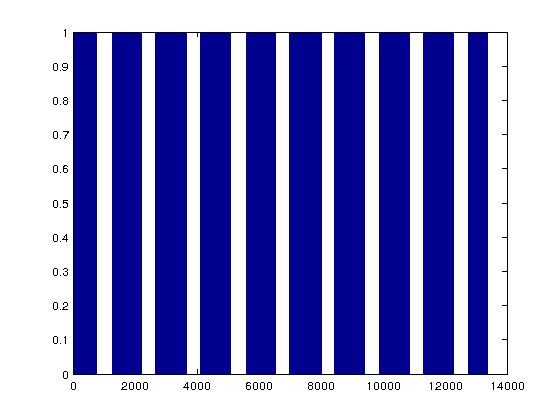
\includegraphics[scale=0.5]{Images/SW.png}}
\caption{Illustration of the opening-closing}
\end{figure}

\begin{figure}[H]
\centering
\begin{tabular}{|c|c|}
\hline
Variable & Value \\
\Ghline
$alpha$ & 1 \\
$L_p$ & 60+1 \\
$h_s$ & 8 \\
$percentile$ & 33 \\
\hline
\end{tabular}
\caption{Parameters values}
\end{figure}

\subsection{Learning stage}

\paragraph{}
The output $y_e(n)$ of the previous stage is an estimate of the final output. It has the right number of transitions but the exact times of these transitions is not precisely determined. The aim of the processing stage is to make those transition times more precise.

\paragraph{}
In order to achieve this objective, a learning is made on the actigraphic data and $y_e(n)$. Only the data 'far' from the estimated transitions, i.e. at least 1 hour before or after a transition, are used. In this way, there are few risks to learn from mislabelled data. These data are then divided into 5-minute windows.

\begin{figure}[h]
\centering
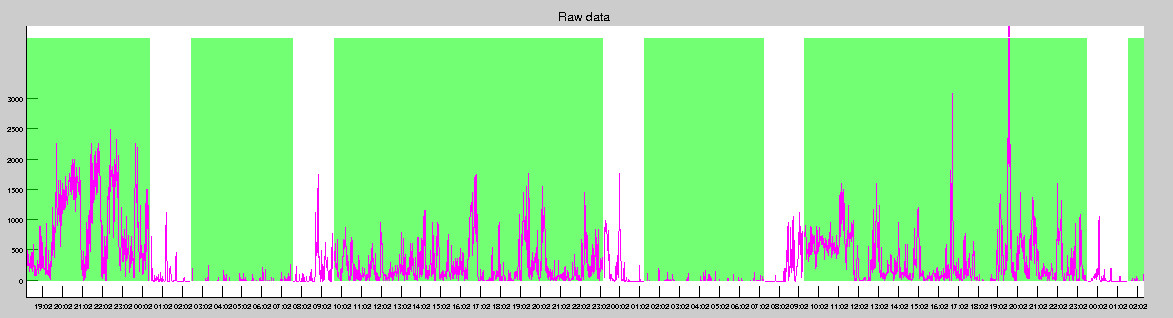
\includegraphics[scale=0.25]{Images/validData.jpg}
\label{valid}
\caption{Raw actigraphic data - The green rectangles show the data that are almost certainly correctly labelled}
\end{figure}

\begin{figure}[H]
\centering
\subfigure[First 5 minutes]{
\label{5min1}
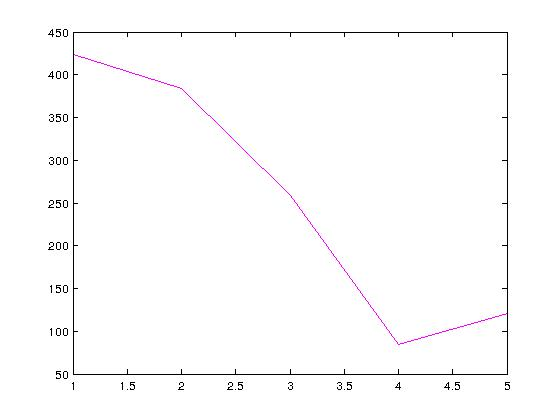
\includegraphics[scale=0.15]{Images/5min1.jpg}
}
\subfigure[Second 5 minutes]{
\label{5min2}
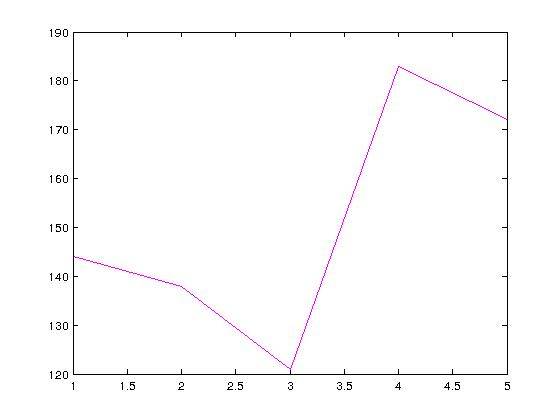
\includegraphics[scale=0.15]{Images/5min2.jpg}
}
\subfigure[Third 5 minutes]{
\label{5min3}
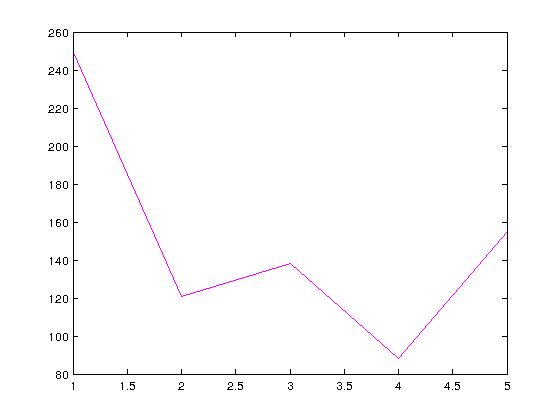
\includegraphics[scale=0.15]{Images/5min3.jpg}
}
\subfigure{
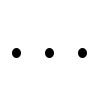
\includegraphics[scale=0.15]{Images/dots.jpg}
}
\caption{The correctly labelled data are divided into 5-minute windows}
\label{5min}
\end{figure}

\paragraph{}
Some features (see Appendix~\ref{sec:extraFeatures}) are then extracted from these windows.

\begin{itemize}
\item The median
\item The interquartile range
\item The mean
\item The standard deviation
\item The maximum
\item The minimum
\item The mode
\item The number of zeros
\end{itemize}

\paragraph{}
This leads to data from which a learning can be made.

\begin{figure}[H]
\centering
\begin{tabular}{cccccccc|c}
\multicolumn{8}{c}{Inputs} & Outputs \\
\multicolumn{8}{c}{$\overbrace{\rule{10cm}{0pt}}$} &  $\overbrace{\rule{2.6cm}{0pt}}$ \\
Median & IQR & Mean & Std Dev & Max & Min & Mode & Zeros & State \\
\hline
212 & 216 & 240 & 135 & 438 & 117 & 117 & 0 & AWAKE \\
337 & 144 & 371 & 137 & 603 & 250 & 250 & 0 & AWAKE \\
\vdots & \vdots & \vdots & \vdots & \vdots & \vdots & \vdots & \vdots & \vdots \\ 
0 & 57 & 44 & 97 & 219 & 0 & 0 & 3 & ASLEEP \\
0 & 0.75 & 0.6 & 1.3 & 3 & 0 & 0 & 4 & ASLEEP \\
\vdots & \vdots & \vdots & \vdots & \vdots & \vdots & \vdots & \vdots & \vdots \\
\end{tabular}
\caption{Example of data on which the learning is applied}
\end{figure}

\paragraph{}
These data are then used to fit the parameters of a neural network by backpropagation (see Appendix~\ref{sec:neuralNetworks}). This neural network will then be used to predict the state of the epoch around the transitions (sleep times and wake times).

\paragraph{}
For every estimated sleep time, a window of one hour before the transition time and one hour after it is studied. A 5-minute sliding window travels along the 2-hour window. For every 5-minute window, the same features as those presented above (median, mean, ...) are extracted. They are entered into the neural network which predicts the state of the window. If the predicted state is ''wake'', the preceding epochs are all set to ''wake''. If the predicted state is ''sleep'', the scoring remains unmodified.

\paragraph{}
The same process is applied to all the wake times : a window of one hour before the transition time and one hour after it is studied. A 5-minute sliding window travels along the 2-hour window. For every 5-minute window, the same features as those presented above (median, mean, ...) are extracted. They are entered into the neural network which predicts the state of the window. If the predicted state is ''sleep'', the preceding epochs are all set to ''sleep''. If the predicted state is ''wake'', the scoring remains unmodified.

\newpage

\section{Results}
\label{sec:results}

\subsection{Experimental data}
\label{subsec:expData}

The algorithm was applied on 25 recordings coming from 25 participants. All of them were young (mean age: 22.73) and healthy. They all fitted the following criteria:
\begin{itemize}
\item \textbf{Clean medical history:} Absence of chronic migraines, epilepsy, neither past severe traumatisms  nor psychiatric or sleep disorders
\item \textbf{No addiction:} Not smoking, no addiction to caffeine (at most 100mg/day) and alchohol (at most 14 unit/week) or chronic medication
\item \textbf{Good quality of life:} Sleep efficiency $> 80\%$, no excessive daytime sleepiness, no signs of anxiety or depression, no night shifts during the last years or travels through more than one time zone during the previous 2 months
\end{itemize}

\paragraph{}
Prior to participating in the laboratory setup of the study, all participants were instructed to keep a regular (fixed) sleep-wake schedule for 7-days. For such, they were requested to keep their bed times and wake times within $\pm$ 15 min, based on their habitual sleep and wake-up times as indexed by the Pittsburgh Sleep Quality Index questionnaire.\\

All the patients wore the actigraph unit on their non-dominant wrist. Every morning, they were also asked to write down their sleep and wake times in a sleep diary.

\paragraph{}
The actigraph used during the study was the Actiwatch L. ''\textit{The Actiwatch-L (AW-L) model is designed to record ambient light levels of 1 to 32,000 lux and movement in the same Actiwatch unit. The AWL has 64k memory is shared equally among storing activity data and light levels and therefore it should be remembered that the maximum recording periods at each epoch are half that of a standard Actiwatch with equivalent memory (i.e. 22 days with a 1 minute epoch). The AWL has no event marker button fitted and is waterproof}''~\cite{Ltd}. The light levels were not used in this study.

\subsection{Results}
\label{subsec:results}
\paragraph{}
The software developped offers 3 differents functions: individual, comparison and group. 
\begin{itemize}
\item The \textbf{individual mode} is the one used when analyzing a single individual for which no human scoring is available. It gives the sleep-wake scoring in a linear form as well as on a circle (see below). It also displays useful informations such as the mean sleep time, the mean sleep duration and so forth. This is the mode that is to be used in a laboratory.

\item The \textbf{comparison mode} is the method used to control the accuracy of the software for a single individual. There must be a manual scoring of this subject available in order to do this comparison. In addition to the data already given in the individual mode, the human scorings are displayed together with the automatic scorings in the linear and the circular forms. Statistical informations such as the error rate, the sensitivity, etc. for the subject are also provided.

\item The \textbf{group mode} is the method used to control the quality of the software for a whole group of individuals. For every subject in the group, there must be a human scoring available. All the statistical data are computed just like done in the comparison mode and the means and extremes (best cases and worst case) are displayed. As additional information, the results of the algorithm are compared with an algorithm that scores the sleep and wake randomly, another one that scores every epoch to wake and a final one that scores every epoch to sleep.

\end{itemize}

\subsubsection{Individual Mode}

\paragraph{}
The first figure displayed (Fig.~\ref{indivLinear}) is the scoring in a linear form. It shows the raw activity with the estimated sleep-wake scoring. The scoring has a value of 1 when the epoch is estimated as wake (the blue bars of the figure) while it has a value of 0 when the epoch is estimated as sleep (the white bars of the figure). MATLAB let the user zoom in and zoom out to get a more precise view. 

\begin{figure}[H]
\centering
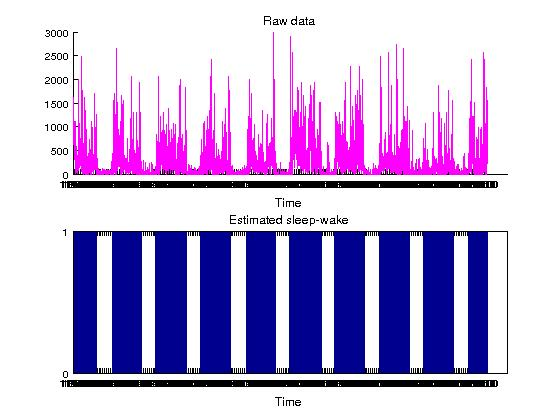
\includegraphics[scale=0.75]{Images/indivResultsLinear.jpg}
\caption{Individual mode applied on a subject - Linear display}
\label{indivLinear}
\end{figure}

\paragraph{}
The second figure (Fig.~\ref{indivCircle}) displays the same data but in another form. The circle represents a '24h-clock'. The 'north' corresponds to midnight, the 'east' to 6AM, the 'south' to noon and the 'west' to 6PM. \\
The data are put on a spiral. The first ''circle'' of the spiral contains the data from the day 1, the second ''circle'' contains the data from the day 2 and so on. The red parts of the spiral are the epochs estimated as wake while the blue parts are the epochs estimated as sleep.

\paragraph{}
The circles on the spiral are the wake and sleep times. Two lines are fitted to these circles in order to obtain a visual estimation of the variability of the sleep of the subject. For this subject, the circular form shows that he woke up roughly at the same time every day but his sleep times are more variable.

\begin{figure}[H]
\centering
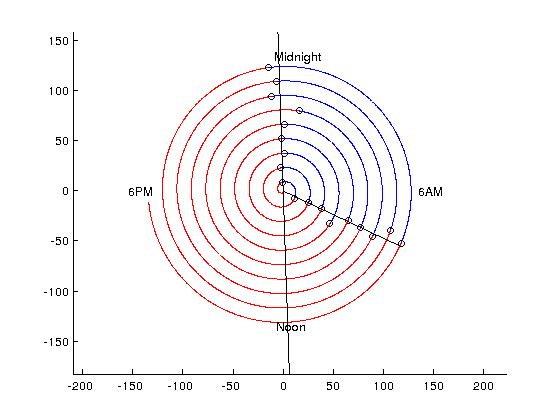
\includegraphics[scale=0.5]{Images/indivResultsCircle.jpg}
\caption{Individual mode applied on a subject - Circular display}
\label{indivCircle}
\end{figure}

\paragraph{}
Finally, statistical information are displayed in MATLAB which are also written in a text file.


\begin{figure}[H]
\centering
\begin{tabular}{|c|c|}
\hline
Variable & Value \\
\Ghline
Mean Wake Time & 06:14 \\
Std Dev Wake Time & 00:51 \\
Mean Sleep Time & 23:58 \\
Std Dev Sleep Time & 01:10 \\
\hline
\end{tabular}
\caption{Individual mode applied on a subject - Statistical data}
\end{figure}


\paragraph{}
For this specific case, we may see that on average, the subject went to sleep at 11:58 PM and woke up at 6:14 AM. We may also see that, as it was assumed from the circular form, the subject has more variability for his sleep time than for his wake time.



\subsubsection{Comparison Mode}

\paragraph{}
The comparison mode displays the same data as the one seen for the individual mode with the addition of the human scoring and a comparison between the two scorings.

\paragraph{}
For the linear form (Fig.~\ref{comparisonLinear}), the raw activity, the automatic scoring, the human scoring and finally, the differences between the two scorings. \\
The ''differences plot'' has a value of 1 when the automatic scoring disagrees with the human scoring (the red bars of the figure) while it has a value of 0 when the two scorings agree (the white bars of the figure).

\begin{figure}[H]
\centering
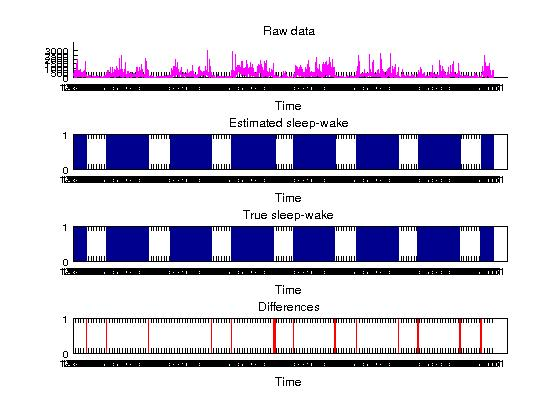
\includegraphics[scale=0.75]{Images/comparisonResultsLinear.jpg}
\caption{Comparison mode applied on a subject - Linear display}
\label{comparisonLinear}
\end{figure}

\paragraph{}
The circular form is the same as the one from the individual mode with the addition of green circles the indicate the wake and sleep times from the human scoring. Two green lines are also fitted to these green circles. \\
The blue/red parts of the spiral still come from the automatic scoring. The only addition of the comparison mode are the green circles and lines.

\begin{figure}[H]
\centering
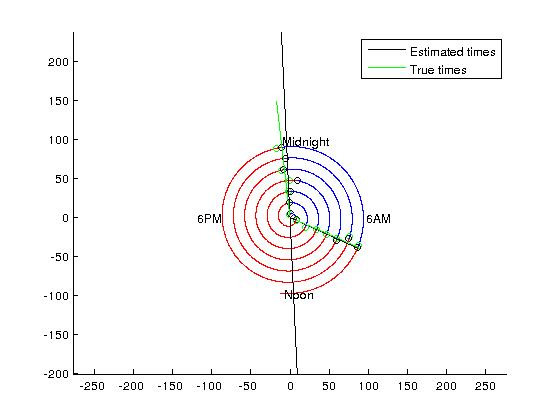
\includegraphics[scale=0.75]{Images/comparisonResultsCircle.jpg}
\caption{Comparison mode applied on a subject - Circular display}
\label{comparisonCircle}
\end{figure}

\paragraph{}
Finally, statistical data are extracted to find how accurate the automate scoring is compared to the human scoring for the chosen subject. First, a confusion matrix is displayed (Fig.~\ref{comparisonMatrix}). From this matrix, some more statistics are extracted (Fig.~\ref{comparisonStats}).

\begin{figure}[H]
\centering
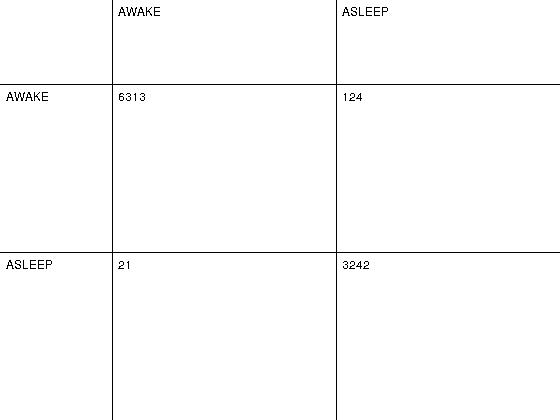
\includegraphics[scale=0.75]{Images/comparisonResultsMatrix.jpg}
\caption{Individual mode applied on a subject - Confusion matrix}
\label{comparisonMatrix}
\end{figure}

\begin{figure}[H]
\centering
\begin{tabular}{|c|c|}
\hline
Variable & Values \\
\Ghline
Error rate & 0.014948\\
Sensitivity & 0.980736 \\
Specificity & 0.993564 \\
Precision & 0.996685 \\
Cohen's Kappa & 0.996685 \\
\hline
\end{tabular}
\caption{Individual mode applied on a subject - Statistics}
\label{comparisonStats}
\end{figure}

\subsubsection{Group Mode}

\paragraph{}
The group mode is the mode used to get statistical data over a group of participants. It was applied on all the participants (see \ref{subsec:expData}) and compared to the following results were obtained :

\begin{figure}[H]
\centering
\begin{tabular}{|c|c|c|c|c|}
\hline
Variable & \textbf{Algorithm} & All Wake & All Sleep & All Random \\
\Ghline
Mean error & \textbf{0.0324} & 0.3484 & 0.6727 & 0.5090 \\
Error worst case & \textbf{0.0689} & 0.3857 & 0.6955  & 0.5173 \\
Error best case & \textbf{0.0126} & 0.3246 & 0.6244  & 0.4967  \\
\hline
Mean sensitivity & \textbf{0.967216} & 0.662678 & X & 0.663282 \\
Sensitivity worst case & \textbf{0.907898} & 0.685490  & X & 0.618039\\
Sensitivity best case & \textbf{0.990152} & 0.624349 & X & 0.689186\\
\hline
Mean specificity & \textbf{0.970623} & X & 0.337322 & 0.337947\\
Specificity worst case & \textbf{0.898429} & X & 0.314510 & 0.318274 \\
Specificity best case & \textbf{0.997551} & X & 0.375651 & 0..369436\\
\hline
Mean Cohen's kappa & \textbf{0.926643} & X & X & X \\
Cohen's kappa worst case & \textbf{0.835390} & X & X & X \\
Cohen's kappa best case & \textbf{0.971820} & X & X & X \\
\hline
\end{tabular}
\caption{Group mode applied on all the participants}
\label{groupStats}
\end{figure}

\newpage

\section{Discussion}

\subsection{Results}

\paragraph{}
These results show that our automatic scoring method is a good alternative to the tedious manual scoring as it provides accurate results with a lot of benefits.

\begin{itemize}
\item \textbf{Automatization:} From the analysis of the data to the writing of the results in a text file, everything is automated and does not require a human intervention. This leads to a process that is much less prone to inadvertent mistakes.

\item \textbf{Execution time:} Our automatic scoring method performs the task faster than a human would. In a couple of minutes, it is able to analyze tens of individuals while it would take up to an hour for a scientist to do the same task. Also, the algorithm only needs a human intervention for its start. Once it is started, the scientist may dedicate his time to other activities.

\item \textbf{Patient-specific:} As explained in the section~\ref{sec:method}, the algorithm is composed of two steps: the processing stage followed by the learning stage. The first stage is a general stage: apart from the threshold, everything is the same for all the data. The second stage, on the other hand, uses features extracted from the actigraphic data that are specific to the inviduals to perfom the learning. Thus this step takes into account that ''being awake'' may be different on a ''activity'' level depending on the individual.

\item \textbf{Objectivity:} The automatic scoring is an objective scoring. That means that uses objective methods to score the data such as a median filtering or a filtering. The manual scoring is a reproducible method. \\ On the other hand, the manual scoring is an extremely subjective method. If he only uses the actigraphic data, the scorer can only make a vague estimation of the sleep and wake times. Which leads to two important drawbacks: the same actigraphic data scored twice by the same person will not give the same manual scoring, neither will the same actigraphic scored by two different persons.
\end{itemize}

\paragraph{}
It has to be noticed that the human scorer bases his scoring on the actigraphic simultaneously with a sleep diary. A sleep diary is a self-reported record of an individual's sleeping and waking times. Thus, if in doubt, the scientist may refer to the sleep diary to perfect his scoring. These data are not available to the automatic method which makes his task harder and more prone to errors. This can explain a part of the inaccuracy in the results of the automatic scoring.

\subsection{Parameters}

\paragraph{}
As already explained in the section~\ref{method}, one of the goal during the implementation of our methods was to develop an algorithm that does not require parameters that are optimized on the dataset. Thus the method that we implemented is a very general one that was developed independtly of the data set. This means that our method should work with other data sets as long as the participants are young and healthy. Moreover nothing seems to prevent the use of our method with studies using another actigraph unit that the one we use (Actiwatch-L). Unfortunately, all the data sets at our disposal were recorder by the same actigraph unit which wouldn't let us confirmed this possibility.

\paragraph{}
Even though the method was developped as a general method with no optimization of the parameters over the data, it uses some parameters that are valid under some assumptions.

\paragraph{}
$h_s$ is a parameter in the processing stage (see~\ref{subsec:processing}) and is defined as the average duration of sleep per night (in hours). As we worked with actigraphic data from young and healthy participants, it was assumed that a value of 8h for $h_s$ was a good estimation (Crespo made the same assumption in his study and obtained good results). If we were working with patient that suffered from insomnia or other sleep disorders or with old people, this parameter should probably be modified to better fit the average duration of their sleep.

\paragraph{}
At the end of this processing stage, an opening and a closing are performed to remove the small transitions as it is assumed that the participants do not wake up in the middle of the night and that they don't sleep during the day either. These assumptions would not remain true if we were working with unhealthy patients of with participants take naps.

\paragraph{}
In the learning stage, the windows used to refine the estimated scoring are 5 minutes long which mean that only 5 values are used to compute the features of every window. This choice is a trade-off between the risk of errors and the accuracy. \\
With a small window, a small number of values are used to compute the features, thus it may lead to errors as it may happen that a window of 5 minute during the day (thus when the individual is awake) shows very little activity. Thus the window is labelled as ''wake'' but the features are similar to the features of the sleep state. \\
On the other hand, a larger window would decrease this risk be would be less accurate in order to find the exact time when the participants went to sleep of woke up.

\paragraph{}
Finally, still in the learning stage, only one hour before and after the transitions are analyzed to refine the transition time. It is again a tradeoff. Sometimes the estimate is not very accurate thus it would be required to analyze a large window around the transition time to find the real transition time. But when widening this window, the risks of false positive (the risks of finding activities that ''looks like'' the real transition) increases.

\subsection{General remarks}

\paragraph{}
During the development of our algorithm, we tried to follow as much recommandations (see section~\ref{subsec:recommandations}) as possible. Here are the checklists with a $\surd$ symbol when the recommandation was followed during our study.

\begin{figure}[H]
\centering
\begin{tabularx}{\textwidth}{|X|c|}
\hline
& Check \\
\Ghline
\textbf{Device/System Information} & \\
$\bullet$ The name of the device, the specific model, and the name (and location) of the manufacturer & $\surd$\\
\hline
$\bullet$ The placement of the device (non-dominant or dominant wrist, left or right ankle, etc.) & $\surd$\\
\hline
$\bullet$ The measured epoch length, the mode of data collection (e.g., ZCM, TAT, PIM, or TRI), the use of the event marker, and the algorithm or wake sensitivity threshold & \\
\hline
$\bullet$ Justification for the algorithm that is chosen & $\surd$\\
\hline
$\bullet$ The type and version of software used & $\surd$\\
\hline
\textbf{Sleep Diary} & \\
$\bullet$ Type of sleep diary used (e.g., paper, electronic, telephone call) & \\
\hline
$\bullet$ Who completed sleep diary (i.e., parent, child) & $\surd$\\
\hline
$\bullet$ Frequency of diary completion (e.g., at bedtime only, morning and evening) & $\surd$\\
\hline
\textbf{Data Collection and Processing (including Missing Data)} & \\
\hline
$\bullet$ Number of nights of data collection & $\surd$\\
\hline
$\bullet$ Number of weekday and weekend nights (if relevant) & \\
\hline
$\bullet$ Methods used to identify and handle artifact & \\
\hline
$\bullet$ How much data lost due to: & \\
$\;\; \bullet$ Technical failure & \\
$\; \bullet$ Participant non-adherence (to wearing the watch or completing the sleep diary) & \\
$\;\; \bullet$ Artifact & \\
\hline
\textbf{Data variables} & \\
\hline
$\bullet$ Clearly define the variables, including ones automatically calculated by manufacturer scoring programs (e.g., sleep bouts, wake bouts, motionless sleep or immobile time, circadian parameters) & $\surd$\\
\hline
$\bullet$ Clearly define the scoring rules used, using common/standardized names & $\surd$\\
\hline
\end{tabularx}
\caption{Proposed Standard Checklist for Reporting Actigraphy in Pediatric Sleep Research Literature (from~\cite{LisaJ.MeltzerHawleyE.Montgomery-DownsSalvatoreP.Insana2012})}
\label{checklistLisa}
\end{figure}

\begin{figure}[H]
\centering
\begin{tabularx}{\textwidth}{|X|c|}
\hline
& Check \\
\Ghline
\textbf{Instrumentation} & \\
\hline
$\bullet$ The word ‘‘actigraph’’ as a key word & $\surd$\\
\hline
$\bullet$ Copyrighted or registered trademark name of the device, model, and name and location of the manufacturer &  $\surd$\\
\hline
$\bullet$ Placement of the actigraph (nondominant or dominant wrist/ankle) & $\surd$\\
\hline
\textbf{Selection of pertinent variables} & \\
\hline
$\bullet$ Specific sleep, activity, and circadian rhythm variables & $\surd$\\
\hline
$\bullet$ Clear definitions of selected variables & $\surd$\\
\hline
\textbf{Sampling} & \\
\hline
$\bullet$ Data collection environment (home, hospital, or somewhere else) & \\
\hline
$\bullet$ Duration of data collection period & $\surd$\\
\hline
$\bullet$ Number of sleep and activity intervals included (single/mean) & \\
\hline
$\bullet$ Days of the week (by name) & \\
\hline
$\bullet$ Sampling epoch length & $\surd$\\
\hline
\textbf{Data processing and analysis} & \\
\hline
$\bullet$ Description of procedures used for preparing files & \\
\hline
$\bullet$ Description of decision rules made for setting time limits of entire file, setting time intervals, editing raw data, handling missing data, handling of naps prior to bedtime, etc. & $\surd$ \\
\hline
$\bullet$ Scoring reliability procedures and percent agreement & $\surd$\\
\hline
$\bullet$ Name of software, mode, and algorithm used for scoring sleep & $\surd$\\
\hline
\end{tabularx}
\caption{Actigraphy Information Suggested for Inclusion in Research Reports (from~\cite{Berger2008})}
\label{checklistBerger}
\end{figure}

\paragraph{}
The use of a sleep diary was mentionned earlier in the paper but other external data may also be useful for the automatic scoring. For example modern actigraphs may contain additional features such as light sensors or off-wrist detectors~\cite{LisaJ.MeltzerHawleyE.Montgomery-DownsSalvatoreP.Insana2012}. Our method was only based on the actigraphic data but by using these additional data, we may expect an improvement in the results. This was not done in our work.

\paragraph{}
Finally, all the codes implementing the algorithm presented in this paper will be freely distributed. The codes are available at the following address : https://github.com/Migwel/Actigraphy. It is thoroughly commented and is provided together with a README which explains how to use the differents modes presented in the section~\ref{subsec:results}.

%Afficher 2 sets de graphiques : un avec un petit alpha et un avec un big alpha

\newpage

\section{Conclusion}

\paragraph{}
The algorithm that was developped during our study has showned accurate results when tested on real-life actigraphy data. This shows that, as already stated by numerous studies, the automatic scoring of actigraphy data is a reliable method for the estimation of the circadian cycles of healthy individuals. The comparison of automatic scoring and manual scoring showed that the automatic way is almost as good as the manual one without suffering from its drawbacks (need for a scientist, tediousity, ...).

\paragraph{}
However, there is still room for improvement. As our algorithm was only tested on data coming from one type of actigraph unit, it cannot be confirmed that it works with other units. The lack of additionnal data didn't let us conduct more sophisticated tests. \\
Another big information to keep in mind is that all the participants were healthy and had stable circadian rhythms. The automatic scoring of patient suffering from sleep disorders as insomnia is a more laborious task and was not approached in this study. \\
As actigraphy is increasingly used in sleep studies, it is very likely that more methods will be developped that will be more accurate and will manage less ''classical'' individuals.

\paragraph{}
Nevertheless, for the tasks that we wanted to overcome, our method displayed great results and could be used in a real laboratory, making the life of the scientists easier.

\newpage
\section{Appendices}
\appendix

\section{Abbreviations}
\label{sec:abbreviations}
\begin{center}
\begin{tabular}{|l|l|}
\hline
Names & Abbreviations \\
\Ghline
ZC & Zero Crossing \\
TAT & Time Above Threshold \\
PI & Proportional Integration \\
PSG & Polysomnygraphy \\
TST & Total Sleep Time \\
WASO & Wake After Sleep Onset \\
SE & Sleep Efficiency \\
EEG & Electroencephalography \\
\hline
\end{tabular}
\end{center}


\newpage

\section{Morphological operations}
\label{sec:morphology}

\paragraph{}
The definitions presented in this annex come from the Digital Image and Video Processing course given by M. Van Droogenbroeck~\cite{VanDroogenbroeck2013}. First, some concepts from the set theory are explained. They are then transposed to the ''signal field'', which is the field in which they are used in the method introduced in this paper

\paragraph{Translation}
The translate of X by b is given by $\{z \in \mathcal{E}| z = x + b, x \in X \} $ and is noted $X_b$. This translation is illustrated on the figure below :

\paragraph{Erosion}
The erosion of X by the structuring element B is given by $X \ominus B = \{ z \in \mathcal{E} | B_z \subseteq X \}$ which is equivalent to $X \ominus B = \bigcap\limits_{b \in B} X_{-b}$.

\paragraph{Dilation}
The dilation of X by the structuring element B is given by $X \oplus B = \{x + b | x \in X, b \in B\}$ which is equivalent to $X \oplus B = \bigcup\limits_{b \in B} X_b = \bigcup\limits_{x \in X} B_x$.

\paragraph{Opening}
The opening of X by the structuring element B consists of an erosion followed by a dilation by the same element B and is given by $X \circ B = (X \ominus B) \oplus B$ which can also be defined as $X \circ B = \bigcup\{B_z | z \in \mathcal{E}, B_z \subseteq X \}$.

\paragraph{Closing}
The closing of X by the structuring element B consists of a dilation followed by an erosion by the same element B and is given by $X \bullet B = (X \oplus B) \ominus B$ which can also be defined as $X \bullet B = \bigcup\{B_z | z \in \mathcal{E}, B_z \subseteq X \}$.

\paragraph{}
Now, let's transpose these concepts to apply them to the algorithm's output binary signal SW(n).

\paragraph{Translation}
The translate of the function f by b is noted $f_b(n)$ and is given by $f_b(n) = f(n-b), \forall x \in \mathcal{E}$.

\paragraph{Erosion}
The erosion of the function f by B is given by $f \ominus B = \bigwedge\limits_{b \in B}f_b(x)$ where $\bigwedge\limits_{i \in I} f_i$ is the largest lower bound of the family of functions $f_i$ ($i \in I$) and is called the \textit{infinum}.

\paragraph{Dilation}
The dilation of the function f by B is given by $f \oplus B = \bigvee\limits_{b \in B}f_b(x)$ where $\bigvee\limits_{i \in I} f_i$ is the lowest upper bound of the family of functions $f_i$ ($i \in I$) and is called the \textit{supremum}.

\paragraph{Opening}
The opening of the function f by the flat structuring element B consists of an erosion followed by a dilation by the same element B and is given by $f \circ B = (f \ominus B) \oplus B$.

\paragraph{Closing}
The closing of the function f by the flat structuring element B consists of a dilation followed by an erosion by the same element B and is given by $f \bullet B = (f \oplus B) \ominus B$.

\paragraph{}
An illustration of the application of an opening and a closing to a binary signal is illustrated on the Fig.~\ref{morphIllustration}. We can see that the successive application of an opening and of a closing removes the short transitions in the original signal.

\begin{figure}[H]
\centering
\subfigure[Original binary function]{
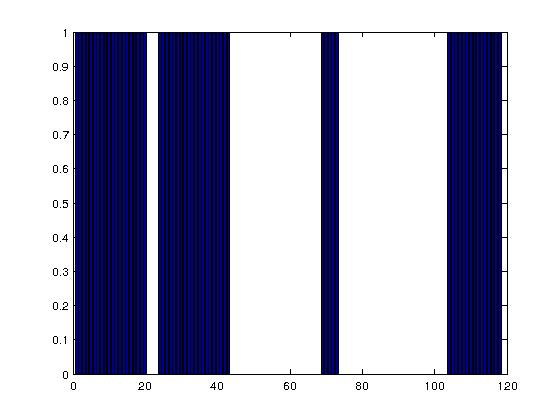
\includegraphics[scale=0.25]{Images/morphSignal.jpg}}
\subfigure[Binary function opened by a 1x15 structuring element]{
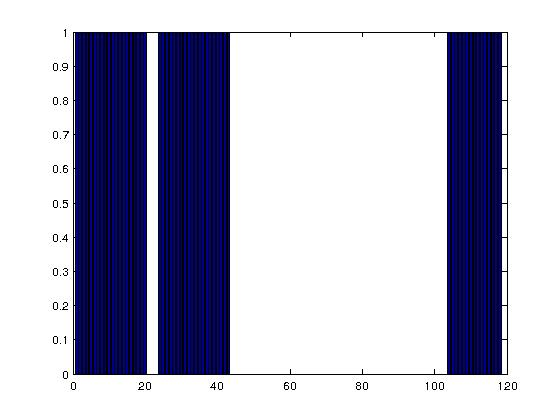
\includegraphics[scale=0.25]{Images/morphOpenedSignal.jpg}}
\subfigure[Binary function opened by a 1x15 structuring element]{
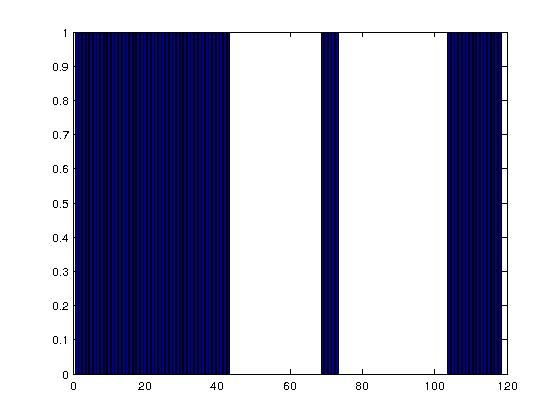
\includegraphics[scale=0.25]{Images/morphClosedSignal.jpg}}
\subfigure[Binary function opened then closed by a 1x15 structuring element]{
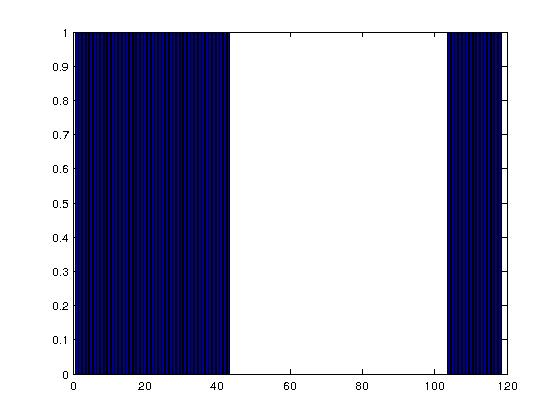
\includegraphics[scale=0.25]{Images/morphFinalSignal.jpg}}
\caption{Morphological operations}
\label{morphIllustration}
\end{figure}

\newpage

\section{Neural Networks}
\label{sec:neuralNetworks}

\paragraph{}
The definition as well as the figures presented in this section come from the Machine Learning course given by L. Wehenkel~\cite{Wehenkel2005}. \\
First, some notations are introduced. Then the perceptron (single-neuron model) is introduced. Finally, the multi-layer perceptron is showed.

\paragraph{}
Neural networks may be used for classification as well as for regression purpose. Since our method only uses a classification neural network, only this case is presented in this section.

\subsection{Notations}

\paragraph{}
\begin{itemize}
\item Learning Sample (observations) : $LS = \{o_1, \ldots, o_N \}$
\item Attribute vector : $\mathbf{a}^i = (a_1(o_i), \ldots, a_n(o_i))^T$
\item Outputs (class) : $c^i = c(o_i) = \pm 1$
\end{itemize}

\subsection{Perceptron}

\begin{figure}[H]
\centering
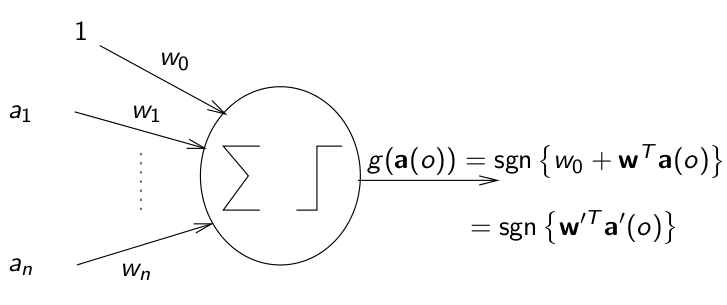
\includegraphics[scale=0.5]{Images/perceptron.png}
\caption{A simple mathematical model of the biological neuron (from~\cite{Wehenkel2005})}
\label{perceptron}
\end{figure}

\paragraph{}
The output fonction $g(\mathbf{a}(o))$ may be the sgn function as shown on the figure~\ref{perceptron} (hard threshold) but more ''complex'' functions may be used as well such as the sigmoid or the hyperbolic tangent (soft threshold).

\subsection{Multi-layers network}

\paragraph{}
Multiple percetrons may then be combined together in layers. Each perceptron in the first layer handles the inputs and its output will be used as an input in the perceptron of the next layer. Finally, a perceptron in the last layer will output a value that is the output value of the neural network.

\begin{figure}[H]
\centering
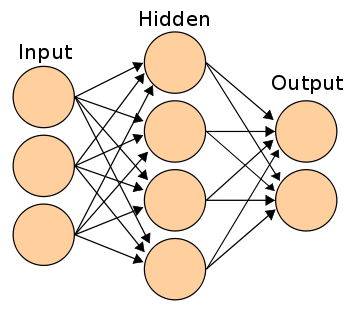
\includegraphics[scale=0.5]{Images/ANN.png}
\caption{Neural Network (from http://www.morosanmihail.com/home/files/2014-05/350px-Artificial\_neural\_network.svg.png)}
\end{figure}

\newpage

\section{Statistical methods}
\label{sec:statMethods}

\paragraph{}
To ascertain that our method was efficient and was as accurate as possible, some statistics were computed and are presented in the section~\ref{sec:results}. Here are their definitions.

\paragraph{Error rate} The error rate is the proportion of epochs that are manually scored as sleep but automatically scored as wake or that are manually scored as wake but automatically scored as sleep.

\paragraph{Sensitivity} The sensitivity is ''\textit{the proportion of epochs [manually] scored as sleep [...] that are accurately identified as sleep by actigraphy.}''\cite{LisaJ.MeltzerHawleyE.Montgomery-DownsSalvatoreP.Insana2012}

\paragraph{Specificity} The specificity is ''\textit{the proportion of [manual]-scored wake epochs accurately identified as wake by actigraphy}''\cite{LisaJ.MeltzerHawleyE.Montgomery-DownsSalvatoreP.Insana2012} \\

\paragraph{Cohen's Kappa} The kappa coefficient is computed as $\kappa = \frac{p_0 - p_e}{1 - p_e}$ where $p_0 = \frac{a + d}{N}$ and $p_e = \frac{(a+c)(a+b) + (b+d)(c+d)}{N^2}$. a, b, c and d are values that come from the confusion matrix, as shown on the figure~\ref{kappa}.

\begin{figure}[H]
\centering
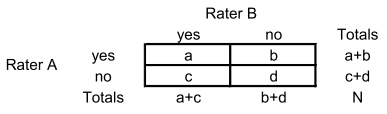
\includegraphics[scale=0.5]{Images/kappa.png}
\caption{Confusion matrix (from~\cite{Cunningham2009})}
\label{kappa}
\end{figure}

\begin{figure}[H]
\centering
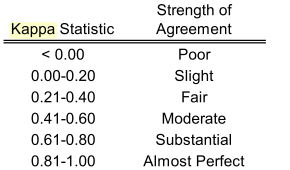
\includegraphics[scale=0.5]{Images/kappa2.png}
\caption{Strength of Agreement using kappa (from~\cite{Cunningham2009})}
\end{figure}

\newpage

\section{Extracted Features}
\label{sec:extraFeatures}

\paragraph{}
The features that are extracted and used for the machine learning are features that are useful in characterizing the signal in the window. They were arbitrarily chosen and proved to be useful to refine the automatic scoring.

\paragraph{Median} The median is the value that separate a set in two halves of the same size: one half where values are larger than the median and the other half in which values are larger than the median. Example: the median of $\{$1, 10, 100, 1000, 10000, 100000, 1000000, 10000000, 100000000, 1000000000$\}$ is 55 000.

\paragraph{Interquartile range} The interquartile range is the range that contains 50\% of the values. They reside between the first quartile, Q1 (the value that is greater than 25\% of all the values of the set and lower than the rest) and the third quartile, Q3 (the value that is lower than 25\% of all the values of the set and greater than the rest). The value that is used for the learning is the difference between Q3 and Q1. Example: the interquartile range of $\{$1, 10, 100, 1000, 10000, 100000, 1000000, 10000000, 100000000, 1000000000$\}$ is $10000000 - 100 =$ 9 999 900.

\paragraph{Mean} The mean is the sum of all the values divided by the number of values in the set. Mathematically, it is expressed as $\frac{1}{N}\sum_{i = 1}^N x_i$ where the $x_i$ are the values of the set of size N. Example: the mean of $\{$1, 10, 100, 1000, 10000, 100000, 1000000, 10000000, 100000000, 1000000000$\}$ is 111 111 111.

\paragraph{Standard Deviation} The standard deviation is a measure of the disparity of the values contained in a set. Mathematically, it is expressed as $\sqrt{\frac{1}{N}\sum_{i = 1}^N (x_i - \mu)^2}$ where the $x_i$ are the values of the set of size N and $\mu$ is the mean of this set. Example: the standard deviation of $\{$1, 10, 100, 1000, 10000, 100000, 1000000, 10000000, 100000000, 1000000000$\}$ is 313 870 000.

\paragraph{Maximum} The maximum of a set of values is the value that has the highest value. Example: the maximum of $\{$1, 10, 100, 1000, 10000, 100000, 1000000, 10000000, 100000000, 1000000000$\}$ is 1000000000.

\paragraph{Minimum} The minimum of a set of values is the value that has the lowest value. Example: the minimum of $\{$1, 10, 100, 1000, 10000, 100000, 1000000, 10000000, 100000000, 1000000000$\}$ is 1.

\paragraph{Mode} The mode is the value that is the most frequent in the set. Example: the mode of $\{$10, 10, 100, 1000, 10000, 100000, 1000000, 10000000, 100000000, 1000000000$\}$ is 1. In MATLAB, if two values share the same amount of occurences, the mode is determine by the value that is the lowest. 


\newpage

\bibliography{biblio}
\bibliographystyle{unsrt}
 
\end{document}


